%% =====================================================================
%%  Capítulo integrado al apunte (2026-10).  El preámbulo, las macros y la
%%  bibliografía viven ahora en main.tex y en referencias.bib.
%% =====================================================================
% =====================================================================

\chapter{Análisis de Componentes Principales (PCA)}\label{cap:pca}

% =====================================================================
\section{Introducción}\label{pca-sec:intro}

El \textbf{Análisis de Componentes Principales} (PCA, por sus siglas en
inglés) es una técnica \emph{no supervisada} para \textbf{reducir la
dimensión} de un conjunto de datos conservando la mayor parte posible de su
variabilidad. Toma $p$ variables, en general \emph{correlacionadas}, y las
reemplaza por $d\le p$ variables nuevas y \emph{no correlacionadas}: las
\emph{componentes principales}, ordenadas de mayor a menor varianza.

PCA se usa de manera transversal en análisis de datos, aprendizaje automático
y visualización, sobre todo con datos de \textbf{alta dimensión} (imágenes,
señales biomédicas, genómica, texto vectorizado), donde sirve para
\emph{resumir} información redundante y filtrar ruido, \emph{visualizar}
estructura en dos o tres dimensiones (PC1 contra PC2) y \emph{acelerar} y
\emph{estabilizar} los modelos que se ajustan después. Un ejemplo típico son
las imágenes de alta resolución: la matriz de intensidades contiene
información redundante, y una aproximación de rango bajo la comprime sin que
el ojo note la diferencia.

Como ya conocemos la SVD, empezamos por la pregunta más fácil de formular:
\begin{center}
\emph{dada una matriz $X$, ¿cuál es la matriz de rango $\le d$ más cercana a $X$?}
\end{center}
La respuesta es el \textbf{teorema de Eckart--Young}: la SVD truncada. La
pregunta de PCA,
\begin{center}
\emph{¿cuál es el subespacio de dimensión $d$ que mejor aproxima a una nube de
puntos de $\R^p$?},
\end{center}
resulta ser un caso particular de la primera, y su solución sale de
Eckart--Young casi gratis. El plan es el siguiente.
\begin{enumerate}[leftmargin=*,itemsep=1pt]
\item Repasamos las normas de matrices que vamos a usar: Frobenius,
espectral y nuclear, y la SVD truncada
(Secciones~\ref{pca-sec:normas} y~\ref{pca-sec:truncada}).
\item Probamos el teorema de Eckart--Young: entre \emph{todas} las matrices de
rango $\le d$, la más cercana a $X$ es la SVD truncada $X_d$
(Sección~\ref{pca-sec:EY}). Es la deuda que quedó pendiente en el capítulo de
la SVD. Enseguida lo vemos funcionar en una foto (Sección~\ref{pca-sec:tigre}).
\item Deducimos la solución del problema de PCA: las direcciones principales
son los primeros $d$ vectores singulares derechos de la matriz de datos
(Sección~\ref{pca-sec:pca}).
\item Releemos la solución con los ojos de la estadística: centrado, matriz de
covarianza, máxima varianza, componentes no correlacionadas y proporción de
varianza explicada (Sección~\ref{pca-sec:varianza}).
\item Hacemos un PCA a mano y decimos cómo se calcula en la computadora
(Sección~\ref{pca-sec:practica}).
\end{enumerate}

\begin{remark}[Un poco de historia]
Pearson \cite{Pearson1901} planteó en 1901 el problema de las ``rectas y planos
más cercanos a un sistema de puntos''  (nuestra Sección~\ref{pca-sec:pca}),
y Hotelling \cite{Hotelling1933} lo reformuló en 1933 como maximización de
varianza (nuestra Sección~\ref{pca-sec:varianza}). El teorema de
aproximación por matrices de rango bajo lleva el nombre de Eckart y Young
\cite{EckartYoung1936} (1936), aunque para operadores integrales ya lo había
probado E.~Schmidt en 1907; ver la historia de la SVD de Stewart
\cite{Stewart1993}.
\end{remark}

% =====================================================================
\section{Lo que vamos a usar de las normas}\label{pca-sec:normas}

Para decidir qué matriz está ``más cerca'' de $X$ hay que medir distancias
entre matrices, y eso ya está hecho: la norma de Frobenius se definió en la
Sección~\ref{sec:frobenius}, la espectral en la Sección~\ref{sec:sigma1}, y la
Sección~\ref{sec:tres-normas} las puso a las dos ---y a la nuclear--- en
términos de los valores singulares,
\[
\normdos{A}=\sigma_1,\qquad
\normF{A}=\bigl(\sigma_1^2+\dots+\sigma_r^2\bigr)^{1/2},\qquad
\normnuc{A}=\sigma_1+\dots+\sigma_r ,
\]
y probó que las tres son \emph{ortogonalmente invariantes}
(Definición~\ref{def:ortog-invariante} y Corolario~\ref{coro:tres-invariantes}):
no cambian al multiplicar por matrices ortogonales, porque eso no cambia los
valores singulares. Esa es la propiedad que vamos a usar una y otra vez.

De la norma de Frobenius necesitamos además dos hechos elementales, que
conviene tener a mano escritos en forma matricial.

\begin{proposition}[Lo que hace falta de Frobenius]\label{pca-prop:frobenius}
Sean $X,A,B\in\R^{n\times p}$ y sea
$\langle A,B\rangle_F=\tr(A^TB)=\sum_{i,j}a_{ij}b_{ij}$ el producto interno de
Frobenius de la Sección~\ref{sec:frobenius}.
\begin{enumerate}[label=(\alph*),leftmargin=*]
\item \textbf{Por filas y por columnas.}
\[
\normF{X}^2=\tr(X^TX)=\tr(XX^T)
=\sum_{j=1}^p\|\col_j(X)\|^2=\sum_{i=1}^n\|\fila_i(X)\|^2 .
\]
\item \textbf{Pitágoras.} Si $P\in\R^{n\times n}$ es una proyección ortogonal
($P=P^T=P^2$), entonces
$\normF{X}^2=\normF{PX}^2+\normF{(I-P)X}^2$; y si $P\in\R^{p\times p}$ lo es,
$\normF{X}^2=\normF{XP}^2+\normF{X(I-P)}^2$.
\end{enumerate}
\end{proposition}

\begin{proof}
(a) La entrada $(j,j)$ de $X^TX$ es $\col_j(X)^T\col_j(X)=\|\col_j(X)\|^2$, y
sumando en $j$ queda $\tr(X^TX)=\sum_j\|\col_j(X)\|^2$, que es la suma de
todos los $x_{ij}^2$. La cuenta con $XX^T$ es la misma leída por filas.

(b) Escribimos $X=PX+(I-P)X$. Las dos piezas son ortogonales para el producto
de Frobenius:
\[
\langle PX,(I-P)X\rangle_F=\tr\bigl(X^TP^T(I-P)X\bigr)
=\tr\bigl(X^T(P-P^2)X\bigr)=0 ,
\]
usando $P^T=P$ y $P^2=P$. Desarrollando
$\normF{X}^2=\langle PX+(I-P)X,\ PX+(I-P)X\rangle_F$ desaparece el término
cruzado. El caso de la derecha es igual con $\tr(XP(I-P)X^T)$.
\end{proof}

\begin{remark}[Dos lecturas de la norma de Frobenius]\label{pca-obs:dos-lecturas}
El ítem (a) es el que vamos a usar todo el tiempo y conviene subrayarlo: la
norma de Frobenius al cuadrado de una matriz de datos es \emph{la suma de los
cuadrados de las longitudes de sus filas}, es decir la suma de $\|\bi{x}_i\|^2$
sobre las $n$ observaciones. Medir una matriz en norma de Frobenius es, para
nosotros, medir una nube de puntos.
\end{remark}

% =====================================================================
\section{La SVD truncada}\label{pca-sec:truncada}

La Proposición~\ref{prop:frobenius-sigmas} ---la que dice que
$\normF{X}^2=\sum_k\sigma_k^2$--- es la que conecta
a Frobenius con la SVD, y lo hace de un modo muy concreto: recordemos que
$X=\sigma_1\bi{u}_1\bi{v}_1^T+\dots+\sigma_ru_rv_r^T$ es una suma de
matrices de rango uno \emph{ordenadas por importancia}. Quedarse con los
primeros $d$ sumandos es \emph{truncar} la SVD.

\begin{corollary}[La SVD truncada]\label{pca-cor:truncada}
Sea $X=U\Sigma V^T$ con $\sigma_1\ge\dots\ge\sigma_r>0$ y sea $d\le r$.
Llamamos $U_d\in\R^{n\times d}$, $V_d\in\R^{p\times d}$ a las matrices con las
primeras $d$ columnas de $U$ y de $V$, $\Sigma_d=\diag(\sigma_1,\dots,\sigma_d)$, y
\[
X_d:=U_d\Sigma_dV_d^T=\sigma_1\bi{u}_1\bi{v}_1^T+\dots+\sigma_du_dv_d^T
\qquad\text{(\textbf{SVD truncada} de $X$).}
\]
Entonces:
\begin{enumerate}[label=(\alph*),leftmargin=*]
\item $X_d=XV_dV_d^T=U_dU_d^T X$: es la proyección (por filas) de
$X$ sobre $\gen(\bi{v}_1,\dots,\bi{v}_d)$, y también la proyección (por columnas) sobre
$\gen(\bi{u}_1,\dots,\bi{u}_d)$.
\item $\rango(X_d)=d$.
\item $\normF{X_d}^2=\sigma_1^2+\dots+\sigma_d^2$ y
$\normF{X-X_d}^2=\sigma_{d+1}^2+\dots+\sigma_r^2$.
\item $\normdos{X-X_d}=\sigma_{d+1}$ y $\normnuc{X-X_d}=\sigma_{d+1}+\dots+\sigma_r$
(con $\sigma_{r+1}:=0$).
\end{enumerate}
\end{corollary}

\begin{proof}
(a) Como las $\bi{v}_i$ son ortonormales, $\bi{v}_i^T V_d$ es la fila $i$-ésima de
$I_d$ si $i\le d$ y es cero si $i>d$. Entonces
$XV_d=\sum_{i=1}^r\sigma_iu_i(\bi{v}_i^T V_d)=\sum_{i=1}^d\sigma_iu_ie_i^T
=U_d\Sigma_d$, y multiplicando por $V_d^T$ queda $X_d$. Del mismo modo
$U_d^T X=\Sigma_dV_d^T$.

(b) $X_d=U_d(\Sigma_dV_d^T)$: las columnas de $U_d$ son linealmente
independientes y $\Sigma_dV_d^T$ tiene $d$ filas linealmente
independientes, así que el producto tiene rango $d$.

(c) y (d) $X-X_d=\sum_{i>d}\sigma_iu_iv_i^T=U_{>d}\Sigma_{>d}V_{>d}^T$,
donde $U_{>d}$ y $V_{>d}$ (las columnas restantes) tienen columnas
ortonormales: es una SVD de $X-X_d$, cuyos valores singulares son entonces
$\sigma_{d+1}\ge\dots\ge\sigma_r$. Las tres normas se leen de los valores
singulares. Igual para $X_d$, cuyos valores singulares son
$\sigma_1,\dots,\sigma_d$.
\end{proof}

\begin{remark}[Cuánto se comprime]\label{pca-rem:compresion}
Guardar $X\in\R^{n\times p}$ cuesta $np$ números. Guardar $X_d=U_d\Sigma_dV_d^T$
cuesta $d(n+p+1)$: $d$ columnas de largo $n$, $d$ de largo $p$ y $d$ valores
singulares. Para una imagen de $512\times512$ con $d=20$ son $20\,500$
números contra $262\,144$: menos del $8\%$. La pregunta es si con tan poco se
pierde mucho. Eckart--Young contesta: el error es exactamente el de los
valores singulares descartados, y \emph{ninguna} otra matriz de rango $\le d$
lo hace mejor.
\end{remark}

% =====================================================================
\section{El teorema de Eckart--Young}\label{pca-sec:EY}

Ahora sí, la pregunta del capítulo. Dada $X\in\R^{n\times p}$ y $d$ menor que
su rango, queremos resolver
\begin{equation}\label{pca-eq:EYprob}
\min_{M\in\R^{n\times p},\ \rango(M)\le d}\ \|X-M\| .
\end{equation}
No es un problema de optimización cualquiera: el conjunto de matrices de rango
$\le d$ no es convexo (la suma de dos matrices de rango uno puede tener rango
dos), así que las herramientas habituales no se aplican. Es excepcional que un
problema así tenga una solución explícita, y esta la tiene.

\begin{theorem}[Eckart--Young \cite{EckartYoung1936}]\label{pca-teo:EY}
Sea $X\in\R^{n\times p}$ con valores singulares $\sigma_1\ge\dots\ge\sigma_r>0$
y sea $1\le d<r$. Para toda $M\in\R^{n\times p}$ con $\rango(M)\le d$,
\begin{align}
\normdos{X-M}&\ \ge\ \sigma_{d+1}=\normdos{X-X_d},\label{pca-eq:EY2}\\
\normF{X-M}^2&\ \ge\ \sigma_{d+1}^2+\dots+\sigma_r^2=\normF{X-X_d}^2 .\label{pca-eq:EY}
\end{align}
Es decir, la SVD truncada $X_d$ es una matriz de rango $\le d$ lo más cercana
posible a $X$, en la norma espectral y en la de Frobenius. En Frobenius, si
$\sigma_d>\sigma_{d+1}$, es la única (Observación~\ref{pca-rem:unicidadEY}).
\end{theorem}

La demostración usa dos herramientas. La primera dice cuánto puede estirar $X$
a un vector según dónde esté; es la versión ``con valores singulares'' del
cociente de Rayleigh.

\begin{lema}[Cuánto estira $X$ a un vector]\label{pca-lema:estira}
Sea $X=U\Sigma V^T$ una SVD completa de $X\in\R^{n\times p}$: las columnas
$\bi{v}_1,\dots,\bi{v}_p$ de $V$ forman una base ortonormal de $\R^p$, $X\bi{v}_i=\sigma_iu_i$
para $i\le r$, $X\bi{v}_i=0$ para $i>r$, y convenimos $\sigma_i=0$ para $r<i\le p$.
Para cada $k=1,\dots,p$:
\begin{enumerate}[label=(\alph*),leftmargin=*]
\item si $\bi{w}\in\gen(\bi{v}_1,\dots,\bi{v}_k)$, entonces $\|X\bi{w}\|\ge\sigma_k\|\bi{w}\|$;
\item si $\bi{w}\in\gen(\bi{v}_k,\dots,\bi{v}_p)$, entonces $\|X\bi{w}\|\le\sigma_k\|\bi{w}\|$.
\end{enumerate}
\end{lema}

\begin{proof}
Escribimos $\bi{w}=c_1\bi{v}_1+\dots+c_pv_p$, de modo que $\|\bi{w}\|^2=\sum_ic_i^2$. Como
$X\bi{w}=\sum_{i\le r}c_i\sigma_iu_i$ y los $\bi{u}_i$ son ortonormales,
\[
\|X\bi{w}\|^2=\sum_{i=1}^pc_i^2\sigma_i^2 .
\]
En (a) solo aparecen los $c_i$ con $i\le k$, y para ellos $\sigma_i\ge\sigma_k$:
la suma es $\ge\sigma_k^2\sum_ic_i^2$. En (b) solo aparecen los $c_i$ con
$i\ge k$, y para ellos $\sigma_i\le\sigma_k$.
\end{proof}

Con $k=1$, la parte (b) es $\|X\bi{w}\|\le\sigma_1\|\bi{w}\|$: volvemos a encontrar
$\normdos{X}=\sigma_1$, que es el Teorema~\ref{teo:sigma1}.

La segunda herramienta es puro conteo de dimensiones y no habla de matrices
para nada. La aislamos porque la vamos a usar dos veces.

\begin{lema}[Tres subespacios que se cortan]\label{pca-lema:dimensiones}
Sean $\mathcal U_1,\mathcal U_2,\mathcal U_3$ subespacios de $\R^p$ con
\[
\dim\mathcal U_1+\dim\mathcal U_2+\dim\mathcal U_3\ >\ 2p .
\]
Entonces $\mathcal U_1\cap\mathcal U_2\cap\mathcal U_3\ne\{0\}$: hay un vector
unitario que está en los tres.
\end{lema}

\begin{proof}
De la fórmula de las dimensiones de la suma,
$\dim(\mathcal U+\mathcal U')=\dim\mathcal U+\dim\mathcal U'
-\dim(\mathcal U\cap\mathcal U')$, y de que $\mathcal U+\mathcal U'$ es un
subespacio de $\R^p$, sale
\[
\dim(\mathcal U\cap\mathcal U')\ \ge\ \dim\mathcal U+\dim\mathcal U'-p .
\]
Aplicándola dos veces, primero a $\mathcal U_1\cap\mathcal U_2$ y después a
ese subespacio con $\mathcal U_3$,
\[
\dim(\mathcal U_1\cap\mathcal U_2\cap\mathcal U_3)
\ \ge\ \dim\mathcal U_1+\dim\mathcal U_2+\dim\mathcal U_3-2p\ \ge\ 1 . \qedhere
\]
\end{proof}

La tercera herramienta es una desigualdad clásica para valores singulares, que
sale del lema anterior.

\begin{lema}[Desigualdad de Weyl para valores singulares]\label{pca-lema:weyl}
Sean $A,B\in\R^{n\times p}$, con la convención $\sigma_k(\cdot)=0$ si $k$
supera al rango. Si $i,j\ge1$ e $i+j-1\le p$, entonces
\begin{equation}\label{pca-eq:weyl}
\sigma_{i+j-1}(A+B)\ \le\ \sigma_i(A)+\sigma_j(B) .
\end{equation}
\end{lema}

\begin{proof}
Sea $C=A+B$ y sean $a_1,\dots,a_p$, $b_1,\dots,b_p$ y $c_1,\dots,c_p$ bases
ortonormales de vectores singulares derechos de $A$, $B$ y $C$ (como en el
Lema~\ref{pca-lema:estira}). Los subespacios
\[
\mathcal U_1=\gen(c_1,\dots,c_{i+j-1}),\qquad
\mathcal U_2=\gen(a_i,\dots,a_p),\qquad
\mathcal U_3=\gen(b_j,\dots,b_p)
\]
tienen dimensiones $i+j-1$, $p-i+1$ y $p-j+1$, que suman $2p+1>2p$. Por el
Lema~\ref{pca-lema:dimensiones} hay un vector unitario $\bi{w}$ en los tres.
Entonces, por el Lema~\ref{pca-lema:estira},
(a) para $C$ y (b) para $A$ y para $B$,
\[
\sigma_{i+j-1}(C)\ \le\ \|C\bi{w}\|\ \le\ \|A\bi{w}\|+\|B\bi{w}\|\ \le\ \sigma_i(A)+\sigma_j(B). \qedhere
\]
\end{proof}

\begin{remark}
Weyl probó en 1912 la desigualdad análoga para los autovalores de matrices
simétricas; la versión para valores singulares se demuestra igual
(ver \cite{HornJohnson2013} o \cite{Bhatia1997}). Una consecuencia útil:
con $j=1$ y $B=E$,
$|\sigma_i(A+E)-\sigma_i(A)|\le\normdos{E}$, es decir, \emph{los valores
singulares son estables frente a perturbaciones}: si a los datos se les suma
un ruido $E$, ningún $\sigma_i$ se mueve más que $\normdos{E}$
(Ejercicio~\ref{pca-ej:weyl}).
\end{remark}

\begin{proof}[Demostración del Teorema de Eckart--Young]
Sea $M$ de rango $\le d$; entonces $\sigma_{d+1}(M)=0$. Aplicamos la
desigualdad de Weyl a $A=X-M$ y $B=M$, con $j=d+1$ e $i=1,\dots,r-d$ (de modo
que $i+j-1=d+i\le r\le p$):
\begin{equation}\label{pca-eq:EYpaso}
\sigma_{d+i}(X)=\sigma_{d+i}\bigl((X-M)+M\bigr)
\ \le\ \sigma_i(X-M)+\sigma_{d+1}(M)=\sigma_i(X-M).
\end{equation}
Con $i=1$ queda $\sigma_{d+1}(X)\le\sigma_1(X-M)=\normdos{X-M}$, que
es~\eqref{pca-eq:EY2}. Elevando~\eqref{pca-eq:EYpaso} al cuadrado y sumando en
$i=1,\dots,r-d$,
\[
\sum_{k=d+1}^{r}\sigma_k^2(X)\ \le\ \sum_{i=1}^{r-d}\sigma_i^2(X-M)
\ \le\ \sum_{i\ge1}\sigma_i^2(X-M)=\normF{X-M}^2 ,
\]
que es~\eqref{pca-eq:EY}. Por último, $X_d$ tiene rango $d$ y los errores
$\normdos{X-X_d}=\sigma_{d+1}$ y $\normF{X-X_d}^2=\sum_{k>d}\sigma_k^2$ son los
del Corolario~\ref{pca-cor:truncada}: se alcanzan las cotas.
\end{proof}

\begin{remark}[La demostración del video, en la norma espectral]
Para la norma espectral el argumento es especialmente transparente (es el que
da Strang \cite{Strang2019}): como $\rango(M)\le d$, el espacio nulo $N(M)$
tiene dimensión $\ge p-d$, y $\gen(\bi{v}_1,\dots,\bi{v}_{d+1})$ tiene dimensión $d+1$;
las dimensiones suman más que $p$, así que hay un vector unitario $\bi{w}$ en los
dos (es el Lema~\ref{pca-lema:dimensiones} con $\mathcal U_3=\R^p$). Entonces $(X-M)\bi{w}=X\bi{w}$ y, por el Lema~\ref{pca-lema:estira}(a),
$\normdos{X-M}\ge\|X\bi{w}\|\ge\sigma_{d+1}$. La desigualdad de Weyl es la misma
idea con un subespacio más, lo que permite comparar \emph{todos} los valores
singulares y no solo el primero.
\end{remark}

\begin{remark}[¿Es única la mejor aproximación?]\label{pca-rem:unicidadEY}
En la norma de Frobenius, si $\sigma_d>\sigma_{d+1}$, $X_d$ es la \emph{única}
matriz de rango $\le d$ a distancia mínima de $X$; no lo vamos a demostrar. En
la norma espectral, en cambio, no es única: esa norma solo ``mira'' el mayor
valor singular del error, y hay lugar para mover el resto
(Ejercicio~\ref{pca-ej:no-unica}).
\end{remark}

\begin{remark}[Eckart--Young--Mirsky: todas las normas invariantes]\label{pca-rem:mirsky}
Que el minimizador sea la SVD truncada no es exclusivo de las normas de
Frobenius y espectral. Mirsky \cite{Mirsky1960} probó que para \emph{toda}
norma ortogonalmente invariante (Definición~\ref{def:ortog-invariante})
\[
\min_{\rango(M)\le d}\|X-M\|=\|X-X_d\| .
\]
El minimizador es el mismo; lo que cambia con la norma es el valor mínimo:
$\bigl(\sum_{i>d}\sigma_i^2\bigr)^{1/2}$ en Frobenius, $\sigma_{d+1}$ en la
espectral, $\sum_{i>d}\sigma_i$ en la nuclear. Hay una demostración corta
en \cite{LiStrang2020}. La invariancia es esencial: para la norma $\|A\|_\infty=$ máxima suma de módulos
por fila, que no es ortogonalmente invariante, el teorema es \emph{falso}
(Ejercicio~\ref{pca-ej:norma-inf}).
\end{remark}

\begin{remark}[Otras demostraciones]
El libro de Strang presenta dos demostraciones más para la norma de Frobenius:
una de G.~W.~Stewart, que parte de la SVD de la matriz óptima $M$ (y no de
$X$), y otra de N.~Srebro, que iguala a cero las derivadas de
$E(C,R)=\normF{X-CR}^2$ respecto de los factores $C$ y $R$ de $M=CR$
(Ejercicio~\ref{pca-ej:srebro}).
\end{remark}

% =====================================================================
\section{Un ejemplo: la foto del tigre}\label{pca-sec:tigre}
% =====================================================================

Una imagen en escala de grises es una matriz: la entrada $a_{ij}\in[0,1]$ es
la intensidad del píxel de la fila $i$ y la columna $j$ ($0$ es negro, $1$ es
blanco). La foto del tigre de la Figura~\ref{pca-fig:tigre-svd} es una matriz
$A\in\R^{620\times600}$. Su SVD la escribe como suma de matrices de rango uno,
\[
A=\sigma_1\bi{u}_1\bi{v}_1^T+\sigma_2\bi{u}_2\bi{v}_2^T+\cdots+\sigma_ru_rv_r^T ,
\qquad r=\rango(A)=598,
\]
y la SVD truncada $A_d=\sum_{i\le d}\sigma_iu_iv_i^T$ se queda con los
primeros $d$ términos. Por el Teorema de Eckart--Young, $A_d$ es la mejor
imagen que se puede armar con $d$ ``piezas'' de rango uno.

\begin{figure}[!htb]
\centering
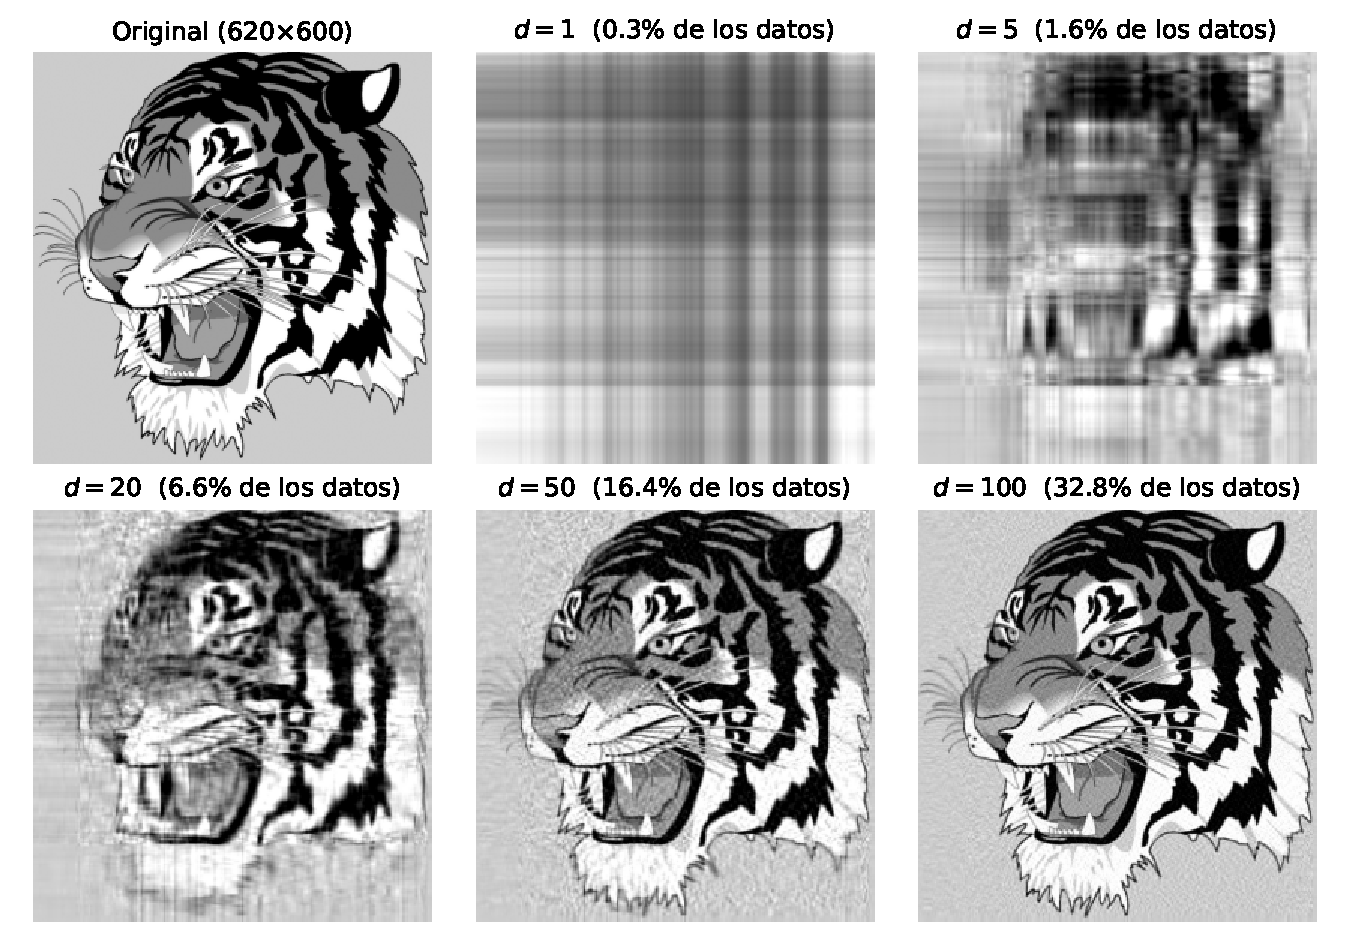
\includegraphics[width=\textwidth]{figuras/I9_tigre_svd.pdf}
\caption{El tigre ($620\times600$; es el dibujo clásico que se distribuye con
Ghostscript, pasado a escala de grises) y sus SVD truncadas $A_d$. Entre
paréntesis, la proporción $d(m+n+1)/(mn)$ de números que hay que guardar.}
\label{pca-fig:tigre-svd}
\end{figure}

\paragraph{Cómo se ve una matriz de rango uno.}
En $A_1=\sigma_1\bi{u}_1\bi{v}_1^T$ la entrada $(i,j)$ es $\sigma_1(\bi{u}_1)_i(\bi{v}_1)_j$:
todas las filas son múltiplos de la misma fila $\bi{v}_1^T$ y todas las
columnas son múltiplos de la misma columna $\bi{u}_1$. Por eso la imagen $d=1$ es
un ``tejido escocés'' de franjas horizontales y verticales, sin ninguna
diagonal. Como $A$ tiene entradas no negativas, $\bi{u}_1$ y $\bi{v}_1$ se pueden
elegir con entradas no negativas (Perron--Frobenius aplicado a $A^T A$),
y $A_1$ es esencialmente el ``gris promedio'' de la foto modulado por filas y
columnas. Ese primer término solo ya se lleva el $81\%$ de
$\normF{A}^2=\sum\sigma_i^2$; los términos siguientes van agregando bordes y
detalles.

\paragraph{Cuánto se guarda.}
Como vimos en la Observación~\ref{pca-rem:compresion}, guardar $A$ cuesta
$mn=372\,000$ números y guardar $A_d$ cuesta $d(m+n+1)$. Con $d=50$ son
$61\,050$ números, el $16{,}4\%$, y el tigre se reconoce sin problemas; con
$d=20$ (el $6{,}6\%$) ya se ven rayas horizontales y verticales, que son la
huella de las matrices de rango uno.

\paragraph{Las cotas de Eckart--Young, en números.}
Eckart--Young no solo dice que $A_d$ es óptima: dice \emph{cuánto} vale el
error, y lo dice solo en términos de los valores singulares descartados. La
tabla lo verifica para el tigre ($\normF{A}\approx429{,}8$, $\sigma_1\approx387{,}3$).
\begin{center}
\renewcommand{\arraystretch}{1.25}
\begin{tabular}{r|cc|cc|c}
$d$ & $\sigma_{d+1}$ & $\normdos{A-A_d}$ & $\bigl(\sum_{i>d}\sigma_i^2\bigr)^{1/2}$
& $\normF{A-A_d}$ & $\normF{A-A_d}/\normF{A}$\\\hline
$5$   & $46{,}48$ & $46{,}48$ & $147{,}67$ & $147{,}67$ & $0{,}34$\\
$20$  & $17{,}77$ & $17{,}77$ & $96{,}40$  & $96{,}40$  & $0{,}22$\\
$50$  & $9{,}35$  & $9{,}35$  & $65{,}40$  & $65{,}40$  & $0{,}15$\\
$100$ & $5{,}18$  & $5{,}18$  & $42{,}65$  & $42{,}65$  & $0{,}10$
\end{tabular}
\end{center}
También se cumple $\normdos{A-A_d}\le\normF{A-A_d}\le\sqrt{r-d}\,\normdos{A-A_d}$
y, en la norma nuclear, $\normnuc{A-A_d}=\sum_{i>d}\sigma_i$ (por ejemplo
$1041{,}3$ para $d=50$).

\paragraph{Comparación con borrar filas y columnas.}
Otra manera ingenua de ``comprimir'' es quedarse con una fracción $1-c$ de
las filas y de las columnas: se guardan $(1-c)^2mn$ números. Para gastar lo
mismo que la SVD con $d=50$ hay que tomar
\[
(1-c)^2mn=d(m+n+1)\quad\Longrightarrow\quad c=1-\sqrt{\frac{d(m+n+1)}{mn}}\approx 0{,}59 ,
\]
es decir, ¡tirar el $59\%$ de las filas y el $59\%$ de las columnas! La
Figura~\ref{pca-fig:tigre-comp} compara, a igual cantidad de números
guardados, borrar las filas y columnas centrales, borrar filas y columnas al
azar (pintándolas de negro para que la imagen conserve el tamaño), rellenar
cada fila o columna borrada con la vecina conservada más cercana, y la SVD
truncada.

\begin{figure}[!htb]
\centering
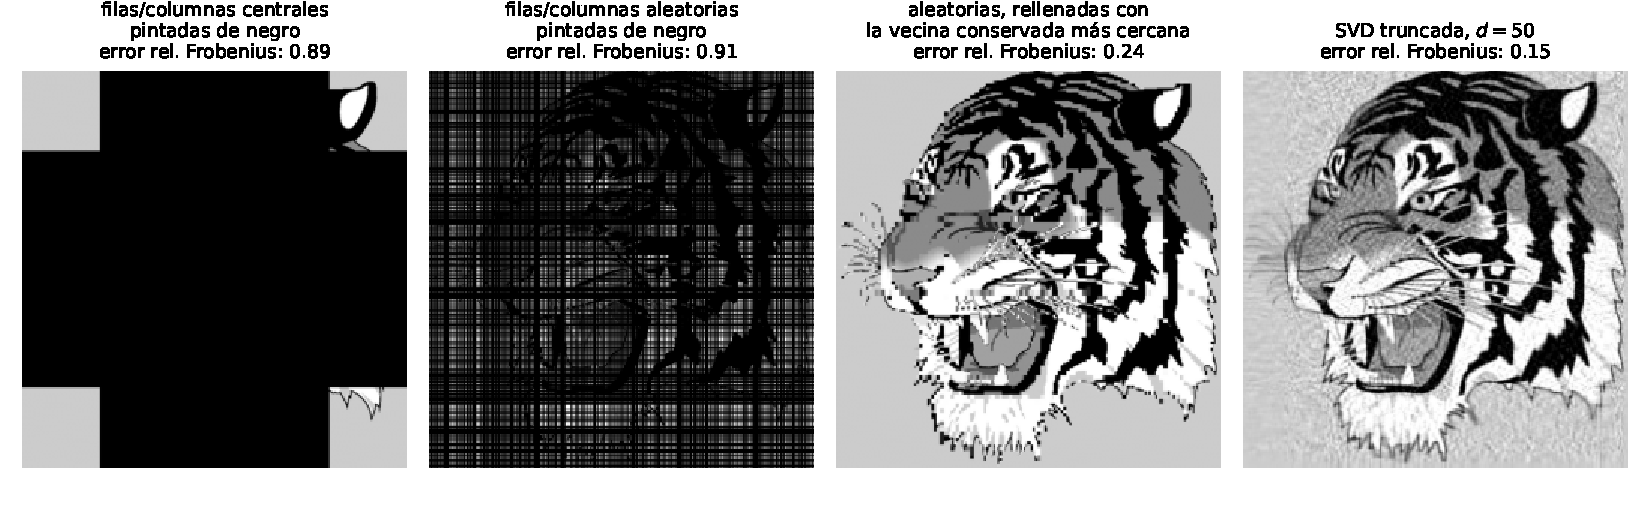
\includegraphics[width=\textwidth]{figuras/I9_tigre_comparacion.pdf}
\caption{Cuatro imágenes que cuestan lo mismo que $A_{50}$
($c\approx59\%$ de filas y columnas descartadas en las tres primeras).}
\label{pca-fig:tigre-comp}
\end{figure}

La SVD gana en las dos normas: el error espectral es $9{,}35$ contra
$19{,}8$ del relleno por vecinos y más de $300$ al pintar de negro; el error
relativo de Frobenius es $0{,}15$ contra $0{,}24$. Y eso a pesar de que la
imagen rellenada tiene rango hasta $243$, mucho más que $50$. Dos
comentarios honestos:
\begin{itemize}[leftmargin=*,itemsep=1pt]
\item Eckart--Young compara $A_d$ con matrices de rango $\le d$; las imágenes
con filas borradas tienen rango mayor, así que el teorema no decide la
comparación: la decide la cuenta.
\item A la vista, la imagen al azar rellenada con la vecina más cercana
parece más nítida que $A_{50}$ aunque esté más lejos en norma. Este tigre es
un dibujo con zonas de gris constante, y duplicar filas vecinas casi no se nota; en cambio la SVD reparte
el error como una textura fina por toda la imagen. Las normas matriciales no
son el ojo humano.
\end{itemize}

\subsection*{¿Se entiende por qué anda tan bien?}

Por Eckart--Young, la pregunta ``¿por qué $A_d$ se parece tanto a $A$?'' es
exactamente la pregunta ``¿por qué los $\sigma_i$ con $i>d$ son tan
chicos?'': el error es $\sigma_{d+1}$ en la norma espectral y
$\bigl(\sum_{i>d}\sigma_i^2\bigr)^{1/2}$ en la de Frobenius. No importa el
rango (el tigre tiene rango $598$, casi completo) sino \emph{la
velocidad con que decaen los valores singulares}.

\begin{figure}[!htb]
\centering
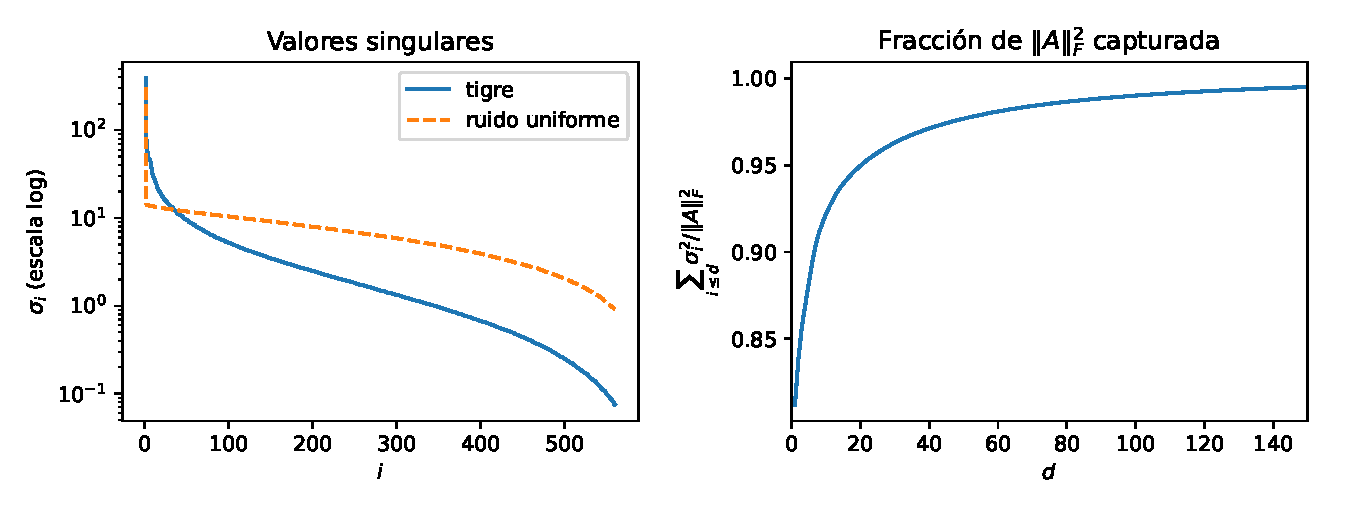
\includegraphics[width=\textwidth]{figuras/I9_tigre_sigmas.pdf}
\caption{Izquierda: valores singulares del tigre y de una matriz de ruido
uniforme en $[0,1]$ del mismo tamaño (escala logarítmica). Derecha: fracción
$\sum_{i\le d}\sigma_i^2/\sum_i\sigma_i^2$ capturada por los primeros $d$
términos, para las dos matrices.}
\label{pca-fig:tigre-sigmas}
\end{figure}

La Figura~\ref{pca-fig:tigre-sigmas} compara el tigre con una matriz ``sin
estructura'': una matriz $R$ de $620\times600$ de \textbf{ruido uniforme}, cuyas
entradas se eligen al azar, independientes y uniformes en $[0,1]$. Es una
``imagen'' de grises sin ninguna relación entre píxeles vecinos. Sus valores
singulares se entienden separando el promedio:
\[
R=\tfrac12\,\mathbf 1\mathbf 1^T+\bigl(R-\tfrac12\,\mathbf 1\mathbf 1^T\bigr).
\]
El primer sumando tiene rango uno y su único valor singular es
$\tfrac12\|\mathbf 1_m\|\,\|\mathbf 1_n\|=\tfrac12\sqrt{mn}\approx305$:
prácticamente el $\sigma_1\approx305{,}1$ de la figura. Solo él ya se lleva el
$75\%$ de $\normF{R}^2$, porque el cuadrado de la media de cada entrada es
$\tfrac14$ y la media de su cuadrado es $\tfrac13$. El segundo sumando tiene
entradas independientes con media $0$ y desvío $1/\sqrt{12}\approx0{,}29$, y
la teoría de matrices aleatorias (la ley de Marchenko--Pastur, y el teorema de Bai--Yin para los
extremos) dice que sus valores singulares llenan el intervalo entre
$(\sqrt m-\sqrt n)/\sqrt{12}\approx0{,}1$ y $(\sqrt m+\sqrt n)/\sqrt{12}\approx14$.
En la figura, $\sigma_2\approx14{,}2$, los $\sigma_i$ bajan lentamente hasta
$\sigma_{560}\approx0{,}9$, y el último es $\sigma_{600}\approx0{,}09$. Sacado el
promedio, la energía queda repartida en cientos de direcciones y no hay nada
que comprimir. La tabla compara las dos matrices (el error relativo es
$\normF{A-A_d}/\normF{A}$, y lo mismo para $R$):
\begin{center}
\renewcommand{\arraystretch}{1.25}
\begin{tabular}{l|c|cc}
& fracción de $\normF{\cdot}^2$ con $d=1$ & error relativo, $d=50$
& error relativo, $d=100$\\\hline
ruido & $75\%$ & $0{,}43$ & $0{,}37$\\
tigre & $81\%$ & $0{,}15$ & $0{,}10$
\end{tabular}
\end{center}
Con $d=1$ las dos se parecen, porque las dos tienen un promedio grande;
después el ruido casi no mejora. En el tigre, en cambio, los $\sigma_i$ caen de
a órdenes de magnitud. Las razones son geométricas:
\begin{itemize}[leftmargin=*,itemsep=1pt]
\item \textbf{Filas vecinas se parecen.} Dos filas consecutivas de una foto
son casi iguales, así que las $620$ filas, vistas como puntos de $\R^{600}$,
están muy cerca de un subespacio de dimensión baja. Esa es justamente la
pregunta de PCA, que viene en la sección siguiente: vamos a ver que
$\normF{A-A_d}^2$ es la suma de las distancias al cuadrado de las filas al mejor
subespacio de dimensión $d$ (Proposición~\ref{pca-prop:distancias}).
\item \textbf{Zonas de color constante tienen rango uno.} Un rectángulo de
gris uniforme es $c\,\mathbf 1\mathbf 1^T$. El fondo y las manchas
grandes cuestan muy poco; lo caro son los bordes.
\item \textbf{Las diagonales son caras.} Un borde diagonal no se alinea con
filas y columnas: la matriz identidad, que es una ``diagonal'', tiene todos
sus valores singulares iguales a $1$ y no se puede comprimir nada
(ver también el Ejercicio~\ref{pca-ej:parabola}). Por
eso los primeros $A_d$ tienen franjas horizontales y verticales y las
diagonales aparecen tarde.
\end{itemize}

\begin{center}
\begin{minipage}{0.85\textwidth}
\centering\emph{Lo que permite comprimir la foto no es el rango sino que sus
valores singulares decaen rápido, y el ruido es justamente el caso en que no
decaen.}
\end{minipage}
\end{center}

\begin{remark}[¿Por qué JPEG no usa la SVD?]
La SVD elige la base óptima \emph{para cada imagen}, pero hay que guardar esa
base: $\bi{u}_i$ y $\bi{v}_i$ son los $d(m+n)$ números del conteo. Los formatos como
JPEG usan una base \emph{fija} (cosenos, en bloques de $8\times8$) que no hay
que transmitir, y guardan solo los coeficientes grandes. La idea es la misma,
con otra base: pocas piezas simples y coeficientes que decaen rápido.
\end{remark}

El Trabajo práctico del final del capítulo propone repetir todo esto con una
foto propia.

% =====================================================================
\section{PCA: la mejor proyección de los datos}\label{pca-sec:pca}

Sea $X\in\R^{n\times p}$ una \textbf{matriz de datos}: $n$ observaciones (las
filas $\bi{x}_1^T,\dots,\bi{x}_n^T$, con $\bi{x}_i\in\R^p$) de $p$ variables (las
columnas). También puede ser una imagen: en el tigre, cada una de las $620$
filas es un punto de $\R^{600}$. Queremos reemplazar cada fila $\bi{x}_i$ por un
punto de un subespacio de dimensión $d\le p$, perdiendo lo menos posible.

\begin{remark}[SVD truncada versus PCA]\label{pca-rem:svd-vs-pca}
Con la foto del tigre aplicamos Eckart--Young directamente a la matriz de
intensidades: queríamos comprimir \emph{esa} matriz. Cuando la matriz es una
tabla de datos, lo que interesa es la \emph{forma} de la nube de puntos, no su
posición: primero \emph{centramos} las variables
(Observación~\ref{pca-rem:origen} y Sección~\ref{pca-sec:varianza}) y después
truncamos. Vamos a ver que PCA es Eckart--Young aplicado a la matriz de datos
centrada.
\end{remark}

Fijemos el subespacio por medio de una base ortonormal: $W\in\R^{p\times d}$
con $W^T W=I_d$ (una matriz \emph{semiortogonal}, en la terminología del
capítulo de Ortogonalidad). Sabemos que $P_W=WW^T$ es la proyección
ortogonal de $\R^p$ sobre $\gen(W)$, el espacio generado por las columnas de
$W$: $P_W$ es simétrica, $P_W^2=P_W$ y $P_W \bi{x}$ es el punto de $\gen(W)$ más
cercano a $\bi{x}$. Reemplazar cada fila $\bi{x}_i$ por su proyección $P_W\bi{x}_i$ es, en
forma matricial, reemplazar $X$ por
\[
XWW^T,\qquad\text{cuya fila $i$ es }(WW^T \bi{x}_i)^T=(P_W\bi{x}_i)^T .
\]
Medimos la pérdida con la norma de Frobenius: sumamos los errores al cuadrado
de todas las entradas.

\begin{definition}[El problema de PCA]\label{pca-def:pca}
Dados $X\in\R^{n\times p}$ y $d\le p$, buscamos
\begin{equation}\label{pca-eq:pca}
\min_{W\in\R^{p\times d},\ W^T W=I_d}\ \normF{X-XWW^T}^2 .
\end{equation}
Las columnas de una solución $W^\ast$ se llaman \textbf{direcciones
principales}; las columnas de $XW^\ast\in\R^{n\times d}$ (las coordenadas de
los datos proyectados) son las \textbf{componentes principales}.
\end{definition}

\begin{proposition}[Qué mide el problema~\eqref{pca-eq:pca}]\label{pca-prop:distancias}
Si $W^T W=I_d$, entonces
\[
\normF{X-XWW^T}^2=\sum_{i=1}^n\|\bi{x}_i-P_W\bi{x}_i\|^2
=\sum_{i=1}^n \dist\bigl(\bi{x}_i,\gen(W)\bigr)^2 .
\]
Es decir, \eqref{pca-eq:pca} pide el subespacio de dimensión $d$ \emph{que pasa
por el origen} y minimiza la suma de los cuadrados de las distancias
(ortogonales) de los datos al subespacio.
\end{proposition}

\begin{proof}
La fila $i$ de $X-XWW^T$ es $\bi{x}_i^T-\bi{x}_i^T WW^T
=(\bi{x}_i-P_W\bi{x}_i)^T$ porque $P_W$ es simétrica. La norma de Frobenius al
cuadrado es la suma de las normas al cuadrado de las filas
(Proposición~\ref{pca-prop:frobenius}(a)). Por último
$\|\bi{x}-P_W\bi{x}\|=\dist(\bi{x},\gen(W))$ es la propiedad básica de la proyección
ortogonal.
\end{proof}

\begin{remark}[Interpretación geométrica: ajuste ortogonal, no regresión]
La recta de regresión de $y$ sobre $\bi{x}$ (la veremos cuando estudiemos mínimos
cuadrados) minimiza distancias \emph{verticales}: el error se mide solo en la
variable respuesta. En~\eqref{pca-eq:pca} no hay variable respuesta: todas
las coordenadas juegan el mismo papel y el error es la distancia
\emph{perpendicular} al subespacio. Por eso PCA es una técnica
\emph{no supervisada}: no usa etiquetas ni distingue entradas de salidas.
\end{remark}

El problema~\eqref{pca-eq:pca} compara a $X$ con matrices de una forma muy
particular, $XWW^T$. Todas ellas tienen rango $\le d$, así que son
candidatas en el problema de Eckart--Young~\eqref{pca-eq:EYprob}: el problema
de PCA es el mismo problema con \emph{menos} competidores. Y el ganador del
problema grande, $X_d=XV_dV_d^T$, ¡es uno de ellos!

\begin{theorem}[Solución de PCA]\label{pca-teo:pca}
Sea $X=U\Sigma V^T$ una SVD completa de $X\in\R^{n\times p}$ (como en el
Lema~\ref{pca-lema:estira}: $V$ es de $p\times p$), con valores
singulares $\sigma_1\ge\dots\ge\sigma_r>0$ (y $\sigma_i=0$ para $i>r$). Para
toda $W\in\R^{p\times d}$ con $W^T W=I_d$,
\[
\normF{X-XWW^T}^2\ \ge\ \sigma_{d+1}^2+\sigma_{d+2}^2+\dots+\sigma_r^2 ,
\]
y la igualdad se alcanza en $W^\ast=V_d$, las primeras $d$ columnas de $V$.
Es decir, las direcciones principales son los primeros $d$ vectores
singulares derechos de $X$, y
\[
\min_{W^T W=I_d}\normF{X-XWW^T}^2
=\min_{\rango(M)\le d}\normF{X-M}^2=\normF{X-X_d}^2 .
\]
\end{theorem}

\begin{proof}
Si $d\ge r$ no hay nada que probar: $XV_dV_d^T=X$ porque $V_d$ contiene a
$\bi{v}_1,\dots,\bi{v}_r$, y el error es cero. Sea $d<r$. Como
$\rango(XWW^T)\le\rango(W)=d$,
\[
\{\,XWW^T:\ W^T W=I_d\,\}\ \subseteq\ \{\,M\in\R^{n\times p}:\ \rango(M)\le d\,\},
\]
y por el Teorema de Eckart--Young,
\[
\normF{X-XWW^T}^2\ \ge\ \min_{\rango(M)\le d}\normF{X-M}^2
=\sum_{i=d+1}^r\sigma_i^2 .
\]
Por otro lado, $W=V_d$ es semiortogonal y $XV_dV_d^T=X_d$
(Corolario~\ref{pca-cor:truncada}(a)), así que
\[
\min_{W^T W=I_d}\normF{X-XWW^T}^2\ \le\ \normF{X-XV_dV_d^T}^2
=\normF{X-X_d}^2=\sum_{i=d+1}^r\sigma_i^2 .
\]
Las dos desigualdades dan la igualdad de los mínimos, alcanzada en $W=V_d$.
\end{proof}

\begin{corollary}[Conclusión práctica]\label{pca-cor:practica}
La mejor proyección de los datos sobre un subespacio de dimensión $d$ usa los
primeros $d$ vectores singulares derechos de $X$:
\begin{itemize}[leftmargin=*]
\item \textbf{direcciones principales}: las columnas $\bi{v}_1,\dots,\bi{v}_d$ de $V_d$;
\item \textbf{datos proyectados}: $\widehat X=XV_dV_d^T=X_d$, la SVD
truncada ($n\times p$, mismo tamaño que $X$, filas en $\gen(V_d)$);
\item \textbf{coordenadas en el subespacio} (\emph{scores}):
$Z=XV_d=U_d\Sigma_d\in\R^{n\times d}$; la fila $i$ de $Z$ son las $d$
coordenadas de $\bi{x}_i$ en la base $\bi{v}_1,\dots,\bi{v}_d$, y $\widehat X=ZV_d^T$.
\end{itemize}
El error cometido es $\normF{X-X_d}^2=\sigma_{d+1}^2+\dots+\sigma_r^2$: la
``energía'' de los valores singulares descartados.
\end{corollary}

\begin{remark}[Qué es único y qué no]\label{pca-rem:unicidad}
Lo que el problema determina es el \emph{subespacio} $\gen(\bi{v}_1,\dots,\bi{v}_d)$,
no la matriz $W$: si $R\in\R^{d\times d}$ es ortogonal, $W=V_dR$ también es
semiortogonal, genera el mismo subespacio, y $WW^T=V_dRR^T V_d^T
=V_dV_d^T$ da el mismo error. En particular cada $\bi{v}_i$ está definido a
menos del signo (una SVD siempre lo está). Si $\sigma_d>\sigma_{d+1}$, el
subespacio óptimo es único (no lo demostramos); si
$\sigma_d=\sigma_{d+1}$ hay infinitos (Ejemplo~\ref{pca-ej:centrar}). Lo que
distingue a la base $V_d$ entre todas las $W=V_dR$ es que sus columnas están
\emph{ordenadas por importancia} y producen componentes \emph{no
correlacionadas} (Teorema~\ref{pca-teo:varianza}).
\end{remark}

\begin{remark}[El origen importa]\label{pca-rem:origen}
El subespacio $\gen(W)$ pasa por el origen. Si la nube de puntos está lejos
del origen, la mejor dirección será la que apunta hacia la nube (hacia su
media) y no la que describe su forma (Ejemplo~\ref{pca-ej:centrar}). Por eso
en la Sección~\ref{pca-sec:varianza} restaremos primero la media de cada
variable. Hasta entonces trabajamos con $X$ genérica: todo lo anterior vale
para cualquier matriz.
\end{remark}

% =====================================================================
\section{PCA como maximización de la varianza}\label{pca-sec:varianza}

Hasta acá resolvimos un problema de aproximación de matrices. Ahora leemos
la solución con los ojos de la estadística ---así se presenta PCA en un curso
de estadística---: aparecen la matriz de covarianza, la varianza de cada
componente y la proporción de varianza explicada. Todo lo que sigue es
\emph{muestral}: no usamos vectores aleatorios ni objetos poblacionales, solo
la tabla de datos.

\subsection{Centrado}

\begin{definition}[Media y matriz centrada]
Sea $X\in\R^{n\times p}$ una matriz de datos. El vector de medias de las
columnas es $\bar{\bi{x}}=\tfrac1n X^T\mathbf 1\in\R^p$, con
$\mathbf 1=(1,\dots,1)^T\in\R^n$, y la \textbf{matriz centrada} es
\[
X_c=X-\mathbf 1\bar{\bi{x}}^T=\Bigl(I-\tfrac1n\mathbf 1\mathbf 1^T\Bigr)X .
\]
Cada columna de $X_c$ tiene media cero: $\mathbf 1^T X_c=0$.
\end{definition}

La matriz $H=I-\frac1n\mathbf 1\mathbf 1^T$ es la proyección ortogonal
sobre $\mathbf 1^\perp$ (es simétrica e idempotente, y $H\mathbf 1=0$): centrar
es proyectar cada columna sobre el complemento ortogonal del vector de unos.

\begin{example}[Por qué hay que centrar]\label{pca-ej:centrar}
Consideremos cuatro observaciones en $\R^2$ ubicadas en los vértices de un
rombo alrededor de $(5,5)$:
\[
X=\begin{pmatrix}6&5\\5&6\\4&5\\5&4\end{pmatrix},\qquad
X^T X=\begin{pmatrix}102&100\\100&102\end{pmatrix},\qquad
\sigma_1^2=202,\ \ \sigma_2^2=2,\ \ \bi{v}_1=\tfrac1{\sqrt2}\begin{pmatrix}1\\1\end{pmatrix}.
\]
Sin centrar, la ``dirección principal'' es la bisectriz, con
$\sigma_1^2/(\sigma_1^2+\sigma_2^2)=99\%$ de la energía: es la dirección que
apunta del origen a la media $(5,5)$, y no dice nada sobre la forma de la nube.
Centrando, $\bar{\bi{x}}=(5,5)^T$ y
\[
X_c=\begin{pmatrix}1&0\\0&1\\-1&0\\0&-1\end{pmatrix},\qquad
X_c^T X_c=\begin{pmatrix}2&0\\0&2\end{pmatrix},\qquad
\sigma_1^2=\sigma_2^2=2 .
\]
La nube centrada es un rombo simétrico: no tiene ninguna dirección
privilegiada, y en efecto \emph{cualquier} vector unitario es una dirección
principal (es el caso $\sigma_1=\sigma_2$ de la Observación~\ref{pca-rem:unicidad}).
\end{example}

\medskip
\noindent\textbf{Convención.} De ahora en más, en esta sección, \emph{$X$
denota la matriz de datos ya centrada por columnas}.

\subsection{Covarianza muestral}

\begin{definition}[Covarianza muestral]
La \textbf{matriz de covarianza muestral} de la matriz centrada
$X\in\R^{n\times p}$ es
\[
S=\frac{1}{n-1}\,X^T X\ \in\R^{p\times p}.
\]
Su entrada $(j,k)$ es $s_{jk}=\frac1{n-1}\sum_{i=1}^nx_{ij}x_{ik}$, la
covarianza muestral entre las variables $j$ y $k$; en la diagonal,
$s_{jj}=\frac1{n-1}\sum_i x_{ij}^2$ es la varianza muestral de la variable
$j$. Las correlaciones son $r_{jk}=s_{jk}/\sqrt{s_{jj}s_{kk}}$.
\end{definition}

\begin{remark}[La letra $S$]\label{pca-obs:letra-S}
En los Capítulos~\ref{cap:sdp} y~\ref{cap:normas} usamos $S$ para una
matriz simétrica definida positiva, la que define un producto interno
$\langle \bi{x},y\rangle_S=\bi{x}^TSy$. Acá $S$ es la covarianza muestral. No es una
coincidencia desafortunada: la Proposición~\ref{pca-prop:S} dice que la
covarianza muestral \emph{es} simétrica semidefinida positiva, y es definida
positiva en cuanto los datos no estén contenidos en un hiperplano por el
origen. O sea que la covarianza muestral es exactamente una de aquellas $S$, y
toda la geometría que construimos con ellas ---la $S$-ortogonalidad, las
$S$-proyecciones, las elipses--- se aplica sin cambiar una coma a la nube de
datos. Volvemos sobre esto en la Sección~\ref{pca-sec:elipse}.
\end{remark}

\begin{proposition}[Propiedades de $S$]\label{pca-prop:S}
Sea $X=U\Sigma V^T$ una SVD completa de la matriz centrada ($V$ de
$p\times p$), con $\sigma_1\ge\dots\ge\sigma_r>0$.
\begin{enumerate}[label=(\alph*),leftmargin=*]
\item $S$ es simétrica y semidefinida positiva: $\bi{w}^T S\bi{w}=\frac1{n-1}\|X\bi{w}\|^2\ge0$.
\item $S=V\Lambda V^T$ con $\Lambda=\frac{1}{n-1}\Sigma^T\Sigma$: los
autovectores de $S$ son los vectores singulares derechos de $X$, y sus
autovalores son
\[
\lambda_k=\frac{\sigma_k^2}{n-1}\quad(k\le r),\qquad \lambda_k=0\quad(k>r).
\]
\item La \textbf{varianza total} es
$\tr(S)=\sum_{j=1}^ps_{jj}=\sum_{k=1}^p\lambda_k=\frac{1}{n-1}\normF{X}^2$.
\end{enumerate}
\end{proposition}

\begin{proof}
(a) $S^T=S$ es inmediato y $\bi{w}^T X^T X\bi{w}=\|X\bi{w}\|^2$.
(b) Como $U^T U=I$,
\[
X^T X=V\Sigma^T U^T U\Sigma V^T=V(\Sigma^T\Sigma)V^T,
\qquad \Sigma^T\Sigma=\diag(\sigma_1^2,\dots,\sigma_r^2,0,\dots,0).
\]
(c) La traza es la suma de la diagonal y también la suma de los autovalores;
la última igualdad es la Proposición~\ref{pca-prop:frobenius}(a).
\end{proof}

\subsection{Error de reconstrucción y varianza explicada}

Dada $W\in\R^{p\times d}$ semiortogonal, las columnas de
\[
Z=XW\in\R^{n\times d}
\]
son $d$ \emph{variables nuevas}: cada una es una combinación lineal de las
$p$ variables originales, con coeficientes en la columna correspondiente de
$W$. La fila $i$ de $Z$ es $\bi{x}_i^T W=(W^T \bi{x}_i)^T$: las
coordenadas de la observación $i$ en la base de $\gen(W)$. Como $X$ está centrada, $Z$ también
($\mathbf 1^T Z=\mathbf 1^T XW=0$), y su matriz de covarianza es
\[
\cov(Z)=\frac{1}{n-1}Z^T Z=W^T SW .
\]
Su traza, $\tr(W^T SW)$, es la varianza total de las variables nuevas: la
\textbf{varianza explicada} por las $d$ direcciones de $W$. El teorema
siguiente dice que error de reconstrucción y varianza explicada son las dos
caras de la misma moneda.

\begin{theorem}[Error de reconstrucción $=$ varianza total $-$ varianza explicada]\label{pca-teo:traza-error}
Sean $X\in\R^{n\times p}$ y $W\in\R^{p\times d}$ con $W^T W=I_d$. Entonces
\begin{equation}\label{pca-eq:traza-error}
\normF{X-XWW^T}^2=\tr(X^T X)-\tr(W^T X^T XW).
\end{equation}
Si $X$ está centrada, dividiendo por $n-1$,
\begin{equation}\label{pca-eq:descomposicion-varianza}
\underbrace{\tr(W^T SW)}_{\text{varianza explicada}}
+\underbrace{\frac{1}{n-1}\normF{X-XWW^T}^2}_{\text{error de reconstrucción}}
=\underbrace{\tr(S)}_{\text{varianza total}} .
\end{equation}
En consecuencia, \emph{minimizar el error de reconstrucción es lo mismo que
maximizar la varianza explicada}, y por el Teorema~\ref{pca-teo:pca} la
solución de los dos problemas es $W^\ast=V_d$.
\end{theorem}

\begin{proof}
Sea $P=WW^T$, que es simétrica e idempotente; entonces $I-P$ también.
Por la Proposición~\ref{pca-prop:frobenius}(a) y la propiedad cíclica de la
traza,
\begin{align*}
\normF{X(I-P)}^2
&=\tr\bigl((I-P)X^T X(I-P)\bigr)
=\tr\bigl(X^T X(I-P)^2\bigr)\\
&=\tr(X^T X)-\tr(X^T XWW^T)
=\tr(X^T X)-\tr(W^T X^T XW).
\end{align*}
La segunda fórmula es la primera dividida por $n-1$, con
$\tr(S)=\tr(X^T X)/(n-1)$. El primer término no depende de $W$, de
donde sigue la equivalencia entre minimizar y maximizar.
\end{proof}

\subsection{Máxima varianza y componentes no correlacionadas}

\begin{theorem}[PCA $=$ máxima varianza explicada]\label{pca-teo:varianza}
Sea $X$ centrada con SVD completa $X=U\Sigma V^T$. Para toda $W\in\R^{p\times d}$
semiortogonal,
\[
\tr(W^T SW)\ \le\ \lambda_1+\dots+\lambda_d ,\qquad \lambda_k=\frac{\sigma_k^2}{n-1},
\]
con igualdad en $W^\ast=V_d$. Las componentes principales
$Z^\ast=XV_d=U_d\Sigma_d$ satisfacen
\[
\cov(Z^\ast)=V_d^T SV_d=\diag(\lambda_1,\dots,\lambda_d):
\]
la $k$-ésima componente principal $z_k=X\bi{v}_k=\sigma_ku_k$ tiene varianza
$\lambda_k=\sigma_k^2/(n-1)$, y componentes distintas están
\textbf{no correlacionadas}.
\end{theorem}

\begin{proof}
Por el Teorema~\ref{pca-teo:traza-error},
$\tr(W^T SW)=\tr(S)-\frac{1}{n-1}\normF{X-XWW^T}^2$, y por el
Teorema~\ref{pca-teo:pca} el error es mínimo en $W=V_d$, donde vale
$\sigma_{d+1}^2+\dots+\sigma_r^2$. Como
$\tr(S)=\frac{1}{n-1}(\sigma_1^2+\dots+\sigma_r^2)$
(Proposición~\ref{pca-prop:S}(c)), el máximo de $\tr(W^T SW)$ es
$\frac{1}{n-1}(\sigma_1^2+\dots+\sigma_d^2)=\lambda_1+\dots+\lambda_d$. La matriz
$V_d^T SV_d=\diag(\lambda_1,\dots,\lambda_d)$ es la
Proposición~\ref{pca-prop:S}(b) restringida a las primeras $d$ columnas.
\end{proof}

Con $d=1$, el teorema es el cociente de Rayleigh del capítulo de la SVD
(Teorema~\ref{teo:rayleigh}) para la matriz $S$:
$\max_{\|\bi{w}\|=1}\bi{w}^T S\bi{w}=\lambda_1$, alcanzado en $\bi{w}=\bi{v}_1$, la dirección de
máxima varianza. Las direcciones siguientes se pueden elegir de a una.

\begin{corollary}[Construcción secuencial: las soluciones están anidadas]\label{pca-cor:anidadas}
Para cada $k$,
\[
\max\{\,\bi{w}^T S\bi{w}:\ \|\bi{w}\|=1,\ \bi{w}\perp \bi{v}_1,\dots,\bi{v}_{k-1}\,\}=\lambda_k ,
\qquad\text{alcanzado en } \bi{w}=\bi{v}_k .
\]
Por lo tanto, la solución del problema con $d$ direcciones, $V_d$, se obtiene
agregando una columna a la solución del problema con $d-1$ direcciones:
\emph{elegir las $d$ mejores direcciones a la vez es lo mismo que elegirlas
de a una}. Esto no es cierto para problemas de optimización arbitrarios, y es
lo que hace tan cómodo al PCA: para pasar de $d$ a $d+1$ no hay que
recalcular nada.
\end{corollary}

\begin{proof}
Si $\|\bi{w}\|=1$ y $\bi{w}\perp \bi{v}_1,\dots,\bi{v}_{k-1}$, la matriz
$W=[\,\bi{v}_1\ \cdots\ \bi{v}_{k-1}\ \bi{w}\,]$ es semiortogonal y, por el
Teorema~\ref{pca-teo:varianza} con $d=k$,
\[
\lambda_1+\dots+\lambda_{k-1}+\bi{w}^T S\bi{w}=\tr(W^T SW)\le\lambda_1+\dots+\lambda_k ,
\]
es decir, $\bi{w}^T S\bi{w}\le\lambda_k$. Con $\bi{w}=\bi{v}_k$ vale la igualdad.
\end{proof}

\begin{remark}[Ortogonal en $\R^p$ $\Longleftrightarrow$ no correlacionado en $\R^n$]
Para direcciones $\bi{w},\bi{w}'\in\R^p$, la covarianza entre las variables $X\bi{w}$ y
$X\bi{w}'$ es $\bi{w}^T S\bi{w}'$. Si $\bi{w}=\bi{v}_k$ es una dirección principal,
$\bi{w}'^T S\bi{v}_k=\lambda_k\,\bi{w}'^T \bi{v}_k$: la variable $X\bi{w}'$ no está
correlacionada con la componente $z_k$ si y solo si $\bi{w}'\perp \bi{v}_k$ (cuando
$\lambda_k\ne0$). Por eso el Corolario~\ref{pca-cor:anidadas} se lee así en el
lenguaje de los datos: \emph{$\bi{v}_1$ es la dirección de máxima varianza; $\bi{v}_2$
es la dirección de máxima varianza entre las no correlacionadas con $z_1$;
$\bi{v}_3$ la de máxima varianza entre las no correlacionadas con $z_1$ y $z_2$},
y así sucesivamente. Las varianzas obtenidas son
$\lambda_1\ge\lambda_2\ge\cdots$.
\end{remark}

\subsection{Proporción de varianza explicada y elección de \texorpdfstring{$d$}{d}}

\begin{definition}[Proporción de varianza explicada]
La \textbf{proporción de varianza explicada} por las primeras $d$ componentes es
\[
\PVE(d)=\frac{\lambda_1+\dots+\lambda_d}{\lambda_1+\dots+\lambda_p}
=\frac{\sigma_1^2+\dots+\sigma_d^2}{\sigma_1^2+\dots+\sigma_r^2}
=\frac{\normF{X_d}^2}{\normF{X}^2}
=1-\frac{\normF{X-X_d}^2}{\normF{X}^2}.
\]
\end{definition}

En la práctica se grafica $\PVE(d)$ (o los $\lambda_k$ en orden decreciente,
el \emph{scree plot}) y se elige $d$ donde la curva hace un ``codo'', o el
menor $d$ que supera un umbral fijado de antemano (típicamente entre $80\%$ y
$95\%$). No hay una regla universal: $d$ es un compromiso entre fidelidad y
simplicidad.

\begin{remark}[Escalas distintas: PCA sobre la matriz de correlación]\label{pca-rem:estandarizar}
El problema~\eqref{pca-eq:pca} suma errores al cuadrado en todas las variables
por igual. Si una variable está en gramos y otra en kilómetros, la de mayor
varianza numérica domina la primera componente aunque no sea la más
informativa. Cuando las unidades no son comparables se \textbf{estandariza}:
se reemplaza $X$ por $X D^{-1/2}$ con $D=\diag(s_{11},\dots,s_{pp})$, de modo
que cada variable pase a tener varianza $1$. La covarianza de la matriz
estandarizada es la matriz de correlación $R=D^{-1/2}SD^{-1/2}$, y su
varianza total es $\tr(R)=p$. Las componentes de $X$ y de $XD^{-1/2}$ son en
general \emph{distintas}: PCA no es invariante por cambios de escala de las
variables (sí lo es por rotaciones: Ejercicio~\ref{pca-ej:rotacion-datos}).
\end{remark}

\begin{remark}[Cómo leer las direcciones principales]
Si llamamos $\bi{x}^{(1)},\dots,\bi{x}^{(p)}\in\R^n$ a las columnas de $X$ (las
variables), la componente $z_k=X\bi{v}_k$ es la variable nueva
$z_k=v_{1k}\bi{x}^{(1)}+\dots+v_{pk}\bi{x}^{(p)}$: una combinación lineal de las
variables originales. Las entradas de $\bi{v}_k$
(\emph{pesos} o \emph{loadings}) dicen qué variables intervienen en la
componente y con qué signo; entradas grandes del mismo signo indican variables
que ``se mueven juntas''. Como $\|\bi{v}_k\|=1$, los pesos son comparables entre
sí, una vez más, solo si las variables están en escalas comparables.
\end{remark}

\begin{remark}[La última componente]
La dirección de \emph{menor} varianza es $\bi{v}_p$, con varianza $\lambda_p$. En
efecto, si $\|\bi{w}\|=1$, la suma de los cuadrados de las distancias de los datos
al hiperplano $\bi{w}^\perp$ es $\|X\bi{w}\|^2=(n-1)\,\bi{w}^T S\bi{w}$, y por el
Teorema~\ref{pca-teo:pca} con $d=p-1$ el hiperplano más cercano a los datos es
$\gen(\bi{v}_1,\dots,\bi{v}_{p-1})=\bi{v}_p^\perp$. Si $\lambda_p\approx0$, los datos están
(casi) contenidos en ese hiperplano: hay una relación lineal aproximada
$v_{1p}\bi{x}^{(1)}+\dots+v_{pp}\bi{x}^{(p)}\approx0$ entre las variables. Es la
\emph{regresión ortogonal} (o de mínimos cuadrados totales).
\end{remark}

\subsection{Geometría en el plano}

Las figuras siguientes muestran $n=60$ observaciones de $p=2$ variables (ya
centradas). Sus valores singulares son $\sigma_1=15{,}03$ y $\sigma_2=3{,}88$, de
modo que $\lambda_1=3{,}83$, $\lambda_2=0{,}26$ y $\PVE(1)=93{,}7\%$.
La Figura~\ref{pca-fig:pca2d}(a) muestra la nube y las dos direcciones
principales; (b) la proyección de cada punto sobre la recta $\gen(\bi{v}_1)$, que
es la reconstrucción de rango uno $\widehat X=XV_1V_1^T$, junto con los
segmentos de error $\bi{x}_i-\widehat{\bi{x}}_i$, todos perpendiculares a la recta; (c)
lo mismo sobre la recta $\gen(\bi{v}_2)$: la suma de los cuadrados de los segmentos
pasa de $\sigma_2^2=15{,}1$ a $\sigma_1^2=225{,}9$; y (d) las componentes
principales $Z=XV$, es decir la misma nube en las coordenadas
$(z_1,z_2)$: los ejes quedan alineados con la forma de la nube y las dos
variables nuevas no están correlacionadas.

\begingroup
% ---- coordenadas de la figura (60 puntos, generados con semilla fija) ----
% puntos originales (centrados)
\newcommand{\nubeXY}{0.30/0.39, 1.07/0.40, -0.19/0.03, -0.92/-1.36, -0.30/-0.54, -1.42/-0.97, 0.19/0.81, 2.50/2.43, -0.13/-0.96, -0.54/-0.84, 1.07/1.19, 1.66/-0.31, 0.71/0.17, -1.34/-0.85, -0.09/0.89, 1.44/1.45, -2.04/-1.45, -0.37/-0.43, -3.10/-2.06, -2.53/-0.44, -2.94/-2.08, 0.02/-0.14, -2.11/-1.01, 0.91/0.54, 0.72/0.37, 0.37/-0.50, -4.33/-2.65, -0.50/-0.57, -0.10/0.82, 0.37/0.75, -2.48/-1.51, -0.74/0.07, -1.35/-1.03, -1.48/-0.12, 2.35/1.52, -1.33/-0.36, 0.71/-0.41, 1.90/1.49, -0.19/-1.25, 0.80/-0.88, 0.67/0.26, 0.77/-0.10, -1.97/-1.06, -0.21/1.52, 3.16/1.45, -2.32/-1.83, 1.90/1.39, 0.43/0.68, -0.78/-0.55, 4.16/2.51, 1.56/1.53, -2.04/-0.85, 0.83/-0.15, 1.47/0.92, 0.00/0.08, 1.97/0.55, 0.16/0.34, 1.88/0.63, 2.74/2.46, -0.96/-0.40}
% proyeccion sobre PC1 (reconstruccion rango 1)
\newcommand{\nubeRunoXY}{0.39/0.25, 0.93/0.61, -0.12/-0.08, -1.27/-0.82, -0.46/-0.30, -1.44/-0.94, 0.51/0.33, 2.87/1.86, -0.53/-0.35, -0.76/-0.50, 1.30/0.84, 1.03/0.67, 0.58/0.37, -1.33/-0.86, 0.34/0.22, 1.68/1.09, -2.10/-1.36, -0.46/-0.30, -3.12/-2.03, -1.98/-1.28, -3.01/-1.96, -0.05/-0.03, -1.95/-1.26, 0.89/0.58, 0.67/0.44, 0.03/0.02, -4.26/-2.76, -0.61/-0.40, 0.31/0.20, 0.60/0.39, -2.44/-1.58, -0.49/-0.32, -1.42/-0.92, -1.10/-0.71, 2.34/1.52, -1.10/-0.71, 0.32/0.20, 2.02/1.31, -0.70/-0.46, 0.16/0.11, 0.59/0.38, 0.50/0.32, -1.87/-1.22, 0.55/0.36, 2.89/1.87, -2.47/-1.61, 1.97/1.28, 0.61/0.40, -0.80/-0.52, 4.08/2.65, 1.80/1.17, -1.82/-1.18, 0.52/0.33, 1.45/0.94, 0.04/0.03, 1.64/1.06, 0.27/0.17, 1.61/1.05, 3.05/1.98, -0.86/-0.56}
% proyeccion sobre PC2
\newcommand{\nubeRdosXY}{-0.09/0.14, 0.13/-0.21, -0.07/0.11, 0.35/-0.53, 0.16/-0.24, 0.02/-0.03, -0.32/0.49, -0.37/0.57, 0.40/-0.61, 0.22/-0.34, -0.22/0.35, 0.64/-0.98, 0.13/-0.20, -0.01/0.02, -0.43/0.67, -0.23/0.36, 0.06/-0.09, 0.09/-0.14, 0.02/-0.03, -0.55/0.84, 0.08/-0.12, 0.07/-0.11, -0.16/0.25, 0.02/-0.03, 0.04/-0.07, 0.34/-0.52, -0.07/0.11, 0.11/-0.17, -0.40/0.62, -0.23/0.36, -0.05/0.07, -0.25/0.39, 0.07/-0.10, -0.38/0.59, 0.00/-0.00, -0.23/0.35, 0.40/-0.61, -0.12/0.18, 0.52/-0.80, 0.64/-0.99, 0.08/-0.12, 0.27/-0.42, -0.10/0.16, -0.75/1.16, 0.28/-0.43, 0.15/-0.23, -0.07/0.11, -0.18/0.28, 0.02/-0.03, 0.09/-0.13, -0.24/0.36, -0.22/0.34, 0.32/-0.49, 0.01/-0.02, -0.04/0.06, 0.34/-0.52, -0.11/0.17, 0.27/-0.42, -0.31/0.48, -0.10/0.15}
\newcommand{\nubeSegUno}{0.30/0.39/0.39/0.25, 1.07/0.40/0.93/0.61, -0.19/0.03/-0.12/-0.08, -0.92/-1.36/-1.27/-0.82, -0.30/-0.54/-0.46/-0.30, -1.42/-0.97/-1.44/-0.94, 0.19/0.81/0.51/0.33, 2.50/2.43/2.87/1.86, -0.13/-0.96/-0.53/-0.35, -0.54/-0.84/-0.76/-0.50, 1.07/1.19/1.30/0.84, 1.66/-0.31/1.03/0.67, 0.71/0.17/0.58/0.37, -1.34/-0.85/-1.33/-0.86, -0.09/0.89/0.34/0.22, 1.44/1.45/1.68/1.09, -2.04/-1.45/-2.10/-1.36, -0.37/-0.43/-0.46/-0.30, -3.10/-2.06/-3.12/-2.03, -2.53/-0.44/-1.98/-1.28, -2.94/-2.08/-3.01/-1.96, 0.02/-0.14/-0.05/-0.03, -2.11/-1.01/-1.95/-1.26, 0.91/0.54/0.89/0.58, 0.72/0.37/0.67/0.44, 0.37/-0.50/0.03/0.02, -4.33/-2.65/-4.26/-2.76, -0.50/-0.57/-0.61/-0.40, -0.10/0.82/0.31/0.20, 0.37/0.75/0.60/0.39, -2.48/-1.51/-2.44/-1.58, -0.74/0.07/-0.49/-0.32, -1.35/-1.03/-1.42/-0.92, -1.48/-0.12/-1.10/-0.71, 2.35/1.52/2.34/1.52, -1.33/-0.36/-1.10/-0.71, 0.71/-0.41/0.32/0.20, 1.90/1.49/2.02/1.31, -0.19/-1.25/-0.70/-0.46, 0.80/-0.88/0.16/0.11, 0.67/0.26/0.59/0.38, 0.77/-0.10/0.50/0.32, -1.97/-1.06/-1.87/-1.22, -0.21/1.52/0.55/0.36, 3.16/1.45/2.89/1.87, -2.32/-1.83/-2.47/-1.61, 1.90/1.39/1.97/1.28, 0.43/0.68/0.61/0.40, -0.78/-0.55/-0.80/-0.52, 4.16/2.51/4.08/2.65, 1.56/1.53/1.80/1.17, -2.04/-0.85/-1.82/-1.18, 0.83/-0.15/0.52/0.33, 1.47/0.92/1.45/0.94, 0.00/0.08/0.04/0.03, 1.97/0.55/1.64/1.06, 0.16/0.34/0.27/0.17, 1.88/0.63/1.61/1.05, 2.74/2.46/3.05/1.98, -0.96/-0.40/-0.86/-0.56}
\newcommand{\nubeSegDos}{0.30/0.39/-0.09/0.14, 1.07/0.40/0.13/-0.21, -0.19/0.03/-0.07/0.11, -0.92/-1.36/0.35/-0.53, -0.30/-0.54/0.16/-0.24, -1.42/-0.97/0.02/-0.03, 0.19/0.81/-0.32/0.49, 2.50/2.43/-0.37/0.57, -0.13/-0.96/0.40/-0.61, -0.54/-0.84/0.22/-0.34, 1.07/1.19/-0.22/0.35, 1.66/-0.31/0.64/-0.98, 0.71/0.17/0.13/-0.20, -1.34/-0.85/-0.01/0.02, -0.09/0.89/-0.43/0.67, 1.44/1.45/-0.23/0.36, -2.04/-1.45/0.06/-0.09, -0.37/-0.43/0.09/-0.14, -3.10/-2.06/0.02/-0.03, -2.53/-0.44/-0.55/0.84, -2.94/-2.08/0.08/-0.12, 0.02/-0.14/0.07/-0.11, -2.11/-1.01/-0.16/0.25, 0.91/0.54/0.02/-0.03, 0.72/0.37/0.04/-0.07, 0.37/-0.50/0.34/-0.52, -4.33/-2.65/-0.07/0.11, -0.50/-0.57/0.11/-0.17, -0.10/0.82/-0.40/0.62, 0.37/0.75/-0.23/0.36, -2.48/-1.51/-0.05/0.07, -0.74/0.07/-0.25/0.39, -1.35/-1.03/0.07/-0.10, -1.48/-0.12/-0.38/0.59, 2.35/1.52/0.00/-0.00, -1.33/-0.36/-0.23/0.35, 0.71/-0.41/0.40/-0.61, 1.90/1.49/-0.12/0.18, -0.19/-1.25/0.52/-0.80, 0.80/-0.88/0.64/-0.99, 0.67/0.26/0.08/-0.12, 0.77/-0.10/0.27/-0.42, -1.97/-1.06/-0.10/0.16, -0.21/1.52/-0.75/1.16, 3.16/1.45/0.28/-0.43, -2.32/-1.83/0.15/-0.23, 1.90/1.39/-0.07/0.11, 0.43/0.68/-0.18/0.28, -0.78/-0.55/0.02/-0.03, 4.16/2.51/0.09/-0.13, 1.56/1.53/-0.24/0.36, -2.04/-0.85/-0.22/0.34, 0.83/-0.15/0.32/-0.49, 1.47/0.92/0.01/-0.02, 0.00/0.08/-0.04/0.06, 1.97/0.55/0.34/-0.52, 0.16/0.34/-0.11/0.17, 1.88/0.63/0.27/-0.42, 2.74/2.46/-0.31/0.48, -0.96/-0.40/-0.10/0.15}
\newcommand{\vunoX}{0.839}\newcommand{\vunoY}{0.544}
\newcommand{\vdosX}{-0.544}\newcommand{\vdosY}{0.839}
\newcommand{\nubeZ}{0.47/0.16, 1.11/-0.25, -0.14/0.13, -1.51/-0.64, -0.54/-0.29, -1.72/-0.04, 0.60/0.58, 3.42/0.68, -0.64/-0.73, -0.91/-0.41, 1.55/0.41, 1.23/-1.17, 0.69/-0.24, -1.59/0.02, 0.41/0.80, 2.00/0.43, -2.50/-0.10, -0.55/-0.16, -3.72/-0.04, -2.36/1.01, -3.59/-0.14, -0.06/-0.13, -2.32/0.30, 1.06/-0.04, 0.80/-0.08, 0.04/-0.62, -5.07/0.13, -0.73/-0.20, 0.37/0.74, 0.72/0.43, -2.90/0.09, -0.58/0.46, -1.69/-0.12, -1.31/0.70, 2.79/-0.00, -1.31/0.42, 0.38/-0.73, 2.41/0.22, -0.84/-0.95, 0.19/-1.17, 0.70/-0.14, 0.59/-0.50, -2.23/0.19, 0.65/1.39, 3.44/-0.51, -2.95/-0.27, 2.35/0.13, 0.73/0.33, -0.95/-0.04, 4.86/-0.16, 2.15/0.43, -2.17/0.40, 0.61/-0.58, 1.73/-0.03, 0.05/0.07, 1.95/-0.62, 0.32/0.20, 1.92/-0.50, 3.64/0.57, -1.02/0.18}
\begin{figure}[!htb]
\centering
\begin{tikzpicture}[scale=0.5]
  \draw[->,gray!70] (-5.4,0)--(5.4,0) node[right]{\scriptsize $\bi{x}_1$};
  \draw[->,gray!70] (0,-3.4)--(0,3.4) node[above]{\scriptsize $\bi{x}_2$};
  \draw[dashed,blue!70!black,thick] ($-5.2*(\vunoX,\vunoY)$)--($5.2*(\vunoX,\vunoY)$) node[right]{\scriptsize $\bi{v}_1$};
  \draw[dashed,red!70!black,thick] ($-3.4*(\vdosX,\vdosY)$)--($3.4*(\vdosX,\vdosY)$) node[above]{\scriptsize $\bi{v}_2$};
  \foreach \x/\y in \nubeXY {\fill[orange!85!black] (\x,\y) circle (1.5pt);}
  \node at (0,-4.0) {\small (a) nube centrada y direcciones principales};
\end{tikzpicture}\hfill
\begin{tikzpicture}[scale=0.5]
  \draw[->,gray!70] (-5.4,0)--(5.4,0) node[right]{\scriptsize $\bi{x}_1$};
  \draw[->,gray!70] (0,-3.4)--(0,3.4) node[above]{\scriptsize $\bi{x}_2$};
  \draw[blue!70!black,thick] ($-5.2*(\vunoX,\vunoY)$)--($5.2*(\vunoX,\vunoY)$) node[right]{\scriptsize $\bi{v}_1$};
  \foreach \x/\y/\a/\b in \nubeSegUno {\draw[gray!60,thin] (\x,\y)--(\a,\b);}
  \foreach \x/\y in \nubeXY {\fill[orange!60] (\x,\y) circle (1.2pt);}
  \foreach \x/\y in \nubeRunoXY {\fill[blue!70!black] (\x,\y) circle (1.4pt);}
  \node at (0,-4.1) {\small (b) proyección sobre $\gen(\bi{v}_1)$: error $=\sigma_2^2=15{,}1$};
\end{tikzpicture}

\vspace{6pt}
\begin{tikzpicture}[scale=0.5]
  \draw[->,gray!70] (-5.4,0)--(5.4,0) node[right]{\scriptsize $\bi{x}_1$};
  \draw[->,gray!70] (0,-3.4)--(0,3.4) node[above]{\scriptsize $\bi{x}_2$};
  \draw[red!70!black,thick] ($-3.4*(\vdosX,\vdosY)$)--($3.4*(\vdosX,\vdosY)$) node[above]{\scriptsize $\bi{v}_2$};
  \foreach \x/\y/\a/\b in \nubeSegDos {\draw[gray!60,thin] (\x,\y)--(\a,\b);}
  \foreach \x/\y in \nubeXY {\fill[orange!60] (\x,\y) circle (1.2pt);}
  \foreach \x/\y in \nubeRdosXY {\fill[red!70!black] (\x,\y) circle (1.4pt);}
  \node at (0,-4.1) {\small (c) proyección sobre $\gen(\bi{v}_2)$: error $=\sigma_1^2=225{,}9$};
\end{tikzpicture}\hfill
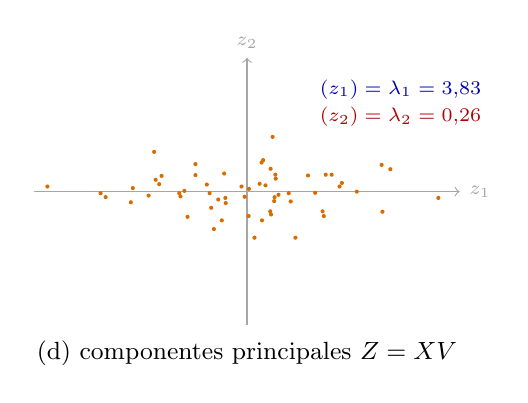
\begin{tikzpicture}[scale=0.5]
  \draw[->,gray!70] (-5.4,0)--(5.4,0) node[right]{\scriptsize $z_1$};
  \draw[->,gray!70] (0,-3.4)--(0,3.4) node[above]{\scriptsize $z_2$};
  \foreach \x/\y in \nubeZ {\fill[orange!85!black] (\x,\y) circle (1.5pt);}
  \node[anchor=west,blue!70!black] at (1.6,2.6) {\scriptsize $\var(z_1)=\lambda_1=3{,}83$};
  \node[anchor=west,red!70!black] at (1.6,1.9) {\scriptsize $\var(z_2)=\lambda_2=0{,}26$};
  \node at (0,-4.1) {\small (d) componentes principales $Z=XV$};
\end{tikzpicture}
\caption{PCA de una nube de $60$ puntos en el plano. (a)~Datos centrados con
$\bi{v}_1$ (azul) y $\bi{v}_2$ (rojo). (b)~Reconstrucción de rango uno $\widehat X=XV_1V_1^T$:
cada punto va a su proyección ortogonal sobre la recta $\gen(\bi{v}_1)$; los
segmentos grises son los errores. (c)~La misma construcción con $\bi{v}_2$: el
error es quince veces mayor. (d)~Las componentes principales: la nube
expresada en la base $\bi{v}_1,\bi{v}_2$; las variables nuevas tienen covarianza cero.}
\label{pca-fig:pca2d}
\end{figure}
\endgroup

% =====================================================================
\subsection{La elipse de la nube}\label{pca-sec:elipse}

Vale la pena detenerse en el dibujo, porque es el mismo que ya hicimos dos
veces. En la Sección~\ref{sec:elipses} vimos que una matriz simétrica definida
positiva $S$ queda retratada por la elipse (o el elipsoide)
\[
\mathcal E=\{\,\bi{x}\in\R^p:\ \bi{x}^TS^{-1}\bi{x}=1\,\} ,
\]
cuyos ejes apuntan en las direcciones de los autovectores de $S$ y cuyos
semiejes miden $\sqrt{\lambda_1},\dots,\sqrt{\lambda_p}$. Si $S$ es la
covarianza muestral de una nube centrada, esa elipse \emph{es} la forma de la
nube: el eje mayor es la dirección en la que los datos se desparraman más.

Juntando las piezas, las direcciones principales $\bi{v}_1,\dots,\bi{v}_p$ son los ejes
de esa elipse, ordenados de mayor a menor semieje, y
$\lambda_k=\sigma_k^2/(n-1)$ son los semiejes al cuadrado. Elegir las $d$
primeras componentes principales es quedarse con los $d$ ejes más largos del
elipsoide y aplastar los demás. Y la elipse explica de un vistazo las dos
advertencias de más arriba: si la nube está lejos del origen la elipse no se
parece en nada a su forma (por eso hay que centrar), y si se cambian las
unidades de una variable el elipsoide se estira en esa dirección y los ejes
giran (por eso hay que estandarizar cuando las unidades no son comparables).

La misma elipse aparece en el Capítulo~\ref{cap:SVD}: por el
Teorema~\ref{teo:elipsoide}, la imagen de la esfera unitaria por una matriz es
un elipsoide de semiejes $\sigma_1,\dots,\sigma_r$ en las direcciones
$\bi{u}_1,\dots,\bi{u}_r$. El elipsoide de los datos y el elipsoide de la SVD son el
mismo objeto mirado desde los dos lados.

% =====================================================================
\section{PCA en la práctica}\label{pca-sec:practica}

\subsection{PCA a mano}

\begin{example}[PCA en $\R^2$, todo a mano]\label{pca-ej:mano}
Tomemos $n=4$, $p=2$ y una matriz \emph{ya centrada} (las columnas suman cero):
\[
X=\begin{pmatrix}2&1\\1&2\\-2&-1\\-1&-2\end{pmatrix}.
\]

\noindent\textbf{1) Covarianza muestral.} Como $n=4$,
\[
S=\frac{1}{n-1}X^T X=\frac13\begin{pmatrix}10&8\\8&10\end{pmatrix}
=\begin{pmatrix}\tfrac{10}{3}&\tfrac{8}{3}\\[2pt]\tfrac{8}{3}&\tfrac{10}{3}\end{pmatrix}.
\]

\medskip
\noindent\textbf{2) Autovalores y autovectores de $S$.} Para una matriz
$\left(\begin{smallmatrix}a&b\\b&a\end{smallmatrix}\right)$ los autovalores
son $a\pm b$, con autovectores $(1,1)^T$ y $(1,-1)^T$. Aquí
\[
\lambda_1=\tfrac{10}{3}+\tfrac{8}{3}=6,\qquad
\lambda_2=\tfrac{10}{3}-\tfrac{8}{3}=\tfrac23,\qquad
\bi{v}_1=\tfrac1{\sqrt2}\begin{pmatrix}1\\1\end{pmatrix},\quad
\bi{v}_2=\tfrac1{\sqrt2}\begin{pmatrix}1\\-1\end{pmatrix}.
\]

\medskip
\noindent\textbf{3) Dirección principal y scores.} Para $d=1$, $W^\ast=\bi{v}_1$ y
la componente principal es $z=X\bi{v}_1$:
\[
z_i=\frac{x_{i1}+x_{i2}}{\sqrt2},\qquad\text{es decir,}\qquad
z=\Bigl(\tfrac{3}{\sqrt2},\ \tfrac{3}{\sqrt2},\ -\tfrac{3}{\sqrt2},\ -\tfrac{3}{\sqrt2}\Bigr)^T .
\]
Su varianza muestral es
$\frac{1}{n-1}\sum_iz_i^2=\frac13\cdot4\cdot\frac92=6=\lambda_1$, como
predice el Teorema~\ref{pca-teo:varianza}. La segunda componente,
$X\bi{v}_2=\frac{1}{\sqrt2}(1,-1,-1,1)^T$, tiene varianza
$\frac13\cdot4\cdot\frac12=\frac23=\lambda_2$ y covarianza cero con $z$.

\medskip
\noindent\textbf{4) Reconstrucción y error (Eckart--Young).} La reconstrucción
de rango uno es $\widehat X=zv_1^T$; fila a fila,
\[
\widehat{\bi{x}}_i=z_i\,\bi{v}_1^T=\pm\tfrac{3}{2}\,(1,1),
\]
de modo que
\[
\normF{X-\widehat X}^2=\sum_{i=1}^4\|\bi{x}_i-\widehat{\bi{x}}_i\|^2
=4\cdot\Bigl(\tfrac14+\tfrac14\Bigr)=2 .
\]
Los valores singulares de $X$ cumplen $\sigma_k^2=(n-1)\lambda_k$:
$\sigma_1^2=18$ y $\sigma_2^2=2$. Eckart--Young predice
$\normF{X-X_1}^2=\sigma_2^2=2$, en perfecto acuerdo con la cuenta directa.

\medskip
\noindent\textbf{5) Varianza total y proporción explicada.}
\[
\tr(S)=\lambda_1+\lambda_2=6+\tfrac23=\tfrac{20}{3},\qquad
\PVE(1)=\frac{6}{20/3}=\frac{18}{20}=0{,}90 .
\]
\textit{Interpretación:} la dirección principal es la bisectriz $x_2=x_1$ (las
dos variables crecen juntas), y quedándonos con una sola coordenada
conservamos el $90\%$ de la variabilidad.
\end{example}

\subsection{PCA en la computadora}

\begin{enumerate}[leftmargin=*,itemsep=1pt]
\item Centrar las columnas de $X$ (y estandarizar si las escalas difieren).
\item Calcular la SVD $X=U\Sigma V^T$.
\item Tomar $W=V_d$. Scores: $Z=XV_d=U_d\Sigma_d$. Reconstrucción:
$\widehat X=ZV_d^T=X_d$.
\item Varianzas $\lambda_k=\sigma_k^2/(n-1)$ y $\PVE(d)$; elegir $d$ mirando el
scree plot o un umbral.
\end{enumerate}
En Python la SVD es la función \texttt{svd} de \texttt{numpy.linalg}, y PCA
ya viene empaquetado en las clases \texttt{PCA} y
\href{https://scikit-learn.org/stable/modules/generated/sklearn.decomposition.TruncatedSVD.html}{\texttt{TruncatedSVD}}
de \texttt{sklearn.decomposition} (esta última no centra: es la SVD truncada
de la Sección~\ref{pca-sec:truncada}).

\begin{remark}[SVD de $X$, no autovalores de $X^T X$]\label{pca-rem:numerica}
Matemáticamente da lo mismo diagonalizar $S$ que calcular la SVD de $X$
(Proposición~\ref{pca-prop:S}). Numéricamente no: formar $X^T X$ eleva al
cuadrado los valores singulares y con ellos el número de condición
$\sigma_1/\sigma_r$, así que los $\sigma_k$ pequeños se pierden en el error de
redondeo. Los programas serios calculan la SVD de la matriz centrada:
\texttt{prcomp} de R siempre, y \texttt{PCA} de \texttt{scikit-learn} salvo
cuando hay pocas variables y muchas más observaciones ($p<1000$ y $n>10p$),
donde por velocidad diagonaliza la covarianza (su documentación advierte que
así es menos estable).
\end{remark}

\begin{remark}[Cuando $p\gg n$: el truco de la matriz de Gram]\label{pca-rem:gram}
Si hay muchas más variables que observaciones (imágenes de $p=10^6$ píxeles,
$n=1000$ fotos), $S$ es de $10^6\times10^6$ pero tiene rango $\le n-1$.
Conviene trabajar con la matriz de Gram $XX^T\in\R^{n\times n}$, cuyos
autovectores son los $\bi{u}_k$ con autovalores $\sigma_k^2$, y recuperar
$\bi{v}_k=X^T \bi{u}_k/\sigma_k$ (ecuación~\eqref{eq:Av-sigma-u} del capítulo de la
SVD). Es lo
que hacen las \emph{eigenfaces} del ejemplo que sigue. Cuando $n$ y $p$ son
ambos enormes se usan métodos iterativos o aleatorizados que solo calculan los
$d$ primeros vectores singulares (\texttt{TruncatedSVD}).
\end{remark}

\subsection{Un ejemplo con muchas variables: las \emph{eigenfaces}}\label{pca-sec:eigenfaces}

Turk y Pentland \cite{TurkPentland1991} usaron PCA para reconocer caras.
Cada foto de $h\times \bi{w}$ píxeles se ``aplana'' en un vector de $\R^{hw}$, y las
$n$ fotos forman las filas de $X\in\R^{n\times hw}$. En la base \emph{Labeled
Faces in the Wild} que usamos en el Trabajo práctico hay $n=1288$ fotos de
$50\times37$ píxeles, así que $p=1850$.
\begin{itemize}[leftmargin=*,itemsep=1pt]
\item La media $\bar{\bi{x}}\in\R^{1850}$ es la \textbf{cara promedio}, y la matriz
centrada $X_c=X-\mathbf 1\bar{\bi{x}}^T$ tiene rango $\le n-1$.
\item Las direcciones principales $\bi{v}_k\in\R^{1850}$ (las filas de $V^T$ en
la SVD de $X_c$) son vectores del mismo tamaño que una foto, y se pueden
\emph{mirar} como imágenes: son las \textbf{eigenfaces}. Las primeras
recogen la iluminación y la forma general de la cara; las siguientes, rasgos
cada vez más finos.
\item Cada cara se aproxima por la cara promedio más una combinación de
pocas eigenfaces,
\[
\bi{x}_i\ \approx\ \bar{\bi{x}}+\sum_{k=1}^dz_{ik}\,\bi{v}_k ,\qquad z_{ik}=\bi{v}_k^T(\bi{x}_i-\bar{\bi{x}}),
\]
que es la fila $i$ de la reconstrucción $\mathbf 1\bar{\bi{x}}^T+(X_c)_d$. En
lugar de $1850$ números, cada cara queda descripta por sus $d$ scores
$(z_{i1},\dots,z_{id})$; con $d$ entre $50$ y $150$ la cara ya se reconoce.
\item Una cara \emph{nueva} $\bi{x}$ se procesa con lo aprendido: se le resta la
misma cara promedio y se proyecta sobre las mismas $\bi{v}_k$.
\end{itemize}

% =====================================================================
\section*{Ejercicios}
\addcontentsline{toc}{section}{Ejercicios}

\noindent\footnotesize Las etiquetas indican el sabor de cada ejercicio:
\textsc{[Cálculo]} para fijar la mecánica, \textsc{[Concepto]} para
justificar y demostrar, \textsc{[Datos]} para la conexión con ciencia de
datos (en la computadora).\normalsize

\begin{enumerate}[leftmargin=*,label=\textbf{\thechapter.\arabic*},ref=\thechapter.\arabic*,itemsep=4pt]

% ---------- normas ----------
\item \tipo{Concepto} \textbf{Proyectar fila a fila.}\label{pca-ej:proyectar} Sea $W\in\R^{p\times d}$
con $W^T W=I_d$ y sea $\Pi_W:\R^{n\times p}\to\R^{n\times p}$,
$\Pi_W(A)=AWW^T$.
\begin{enumerate}[label=(\alph*)]
\item Probar que $\Pi_W$ es lineal, que $\Pi_W\circ\Pi_W=\Pi_W$, y que para
todas las matrices $A,B$ vale
$\langle\Pi_W(A),B\rangle_F=\langle A,\Pi_W(B)\rangle_F$. Es decir, $\Pi_W$
es una proyección ortogonal del espacio de matrices con el producto interno
de Frobenius. ¿Sobre qué subespacio de $\R^{n\times p}$ proyecta?
\item Si las columnas de $W$ son linealmente independientes pero no
ortonormales, ¿cuál es la proyección ortogonal de $\R^p$ sobre $\gen(W)$?
Probar que
\[
\min_{C\in\R^{n\times d}}\normF{X-CW^T}^2
\quad\text{se alcanza en}\quad C=XW(W^T W)^{-1},
\]
y que el mínimo no cambia si se reemplaza $W$ por una base ortonormal del
mismo subespacio.
\end{enumerate}

\item \tipo{Concepto} \textbf{Frobenius y la norma espectral.} Sean
$A\in\R^{m\times n}$ y $B\in\R^{n\times p}$.
\begin{enumerate}[label=(\alph*)]
\item Probar que $\normF{AB}\le\normdos{A}\,\normF{B}$ y que
$\normF{AB}\le\normF{A}\,\normF{B}$. \emph{Ayuda:} mirar $AB$ columna por
columna.
\item Probar que $\normdos{A}\le\normF{A}\le\sqrt{r}\,\normdos{A}$ con
$r=\rango(A)$, y decir para qué matrices vale cada igualdad.
\item Probar que $\normF{A}^2=\sum_i\|A\bi{e}_i\|^2=\sum_i\|A\bi{q}_i\|^2$ para cualquier
base ortonormal $\bi{q}_1,\dots,q_n$ de $\R^n$. (Esto explica por qué Frobenius es
invariante ortogonal.)
\end{enumerate}

\item \tipo{Concepto} \textbf{Normas ortogonalmente invariantes.}\label{pca-ej:invariantes}
\begin{enumerate}[label=(\alph*)]
\item Probar que si $Q$ y $Q'$ son ortogonales, $QAQ'$ tiene los mismos
valores singulares que $A$. \emph{Ayuda:} si $A=U\Sigma V^T$, ¿cuál es
una SVD de $QAQ'$?
\item Deducir que son ortogonalmente invariantes la norma de Frobenius, la
espectral $\normdos{A}=\max_{\|\bi{x}\|=1}\|A\bi{x}\|=\sigma_1(A)$, la nuclear
$\normnuc{A}=\sum_i\sigma_i(A)$ y (opcional) las normas de Ky Fan
$\|A\|_{(k)}=\sum_{i=1}^k\sigma_i(A)$. Para la espectral, dar además una
prueba directa a partir de la definición como máximo.
\item ¿Cuál de las normas de (b) proviene de un producto interno?
\item Calcular las normas de Frobenius, espectral y nuclear de $I_n$ y de la
matriz $\mathbf 1\mathbf 1^T\in\R^{n\times n}$ de todos unos.
\end{enumerate}

\item \tipo{Concepto} \textbf{Consecuencias de la desigualdad de Weyl.}\label{pca-ej:weyl}
Sean $A,B,E\in\R^{n\times p}$.
\begin{enumerate}[label=(\alph*)]
\item Probar que $|\sigma_i(A+E)-\sigma_i(A)|\le\normdos{E}$ para todo $i$.
\emph{Ayuda:} Weyl con $j=1$, aplicada a $A+E$ y a $A=(A+E)+(-E)$.
Interpretar: si a una matriz de datos se le suma un ruido de norma espectral
chica, sus valores singulares casi no cambian.
\item Probar que si $\rango(B)\le k$, entonces $\sigma_{i+k}(A)\le\sigma_i(A+B)$
y $\sigma_{i+k}(A+B)\le\sigma_i(A)$: sumar una matriz de rango $k$ corre los
valores singulares a lo sumo $k$ lugares.
\item Deducir que si $A'$ se obtiene de $A$ cambiando una sola fila, entonces
$\sigma_{i+1}(A)\le\sigma_i(A')\le\sigma_{i-1}(A)$ para todo $i$, con la
convención $\sigma_0(A)=+\infty$ (los valores singulares
\emph{se entrelazan}). Un único dato atípico, ¿puede agrandar mucho a
$\sigma_1$? ¿Y a $\sigma_1$ y $\sigma_2$ a la vez?
\end{enumerate}

% ---------- Eckart–Young ----------
\item \tipo{Concepto} \textbf{Quitar el sumando más grande.} Sea
$A=\sum_{i=1}^r\sigma_iu_iv_i^T$ la SVD de $A$ y $A_k$ su SVD truncada.
\begin{enumerate}[label=(\alph*)]
\item Dar una matriz de rango uno lo más próxima posible a $A$ (en Frobenius y
en la norma espectral). ¿Y de rango $k$? ¿Cuándo es la única posible?
\item ¿Cuáles son los valores singulares (en orden decreciente) de $A-A_k$?
Omitir los ceros. ¿Cuál es su rango?
\item Calcular $\normF{A-A_k}$, $\normdos{A-A_k}$ y $\normnuc{A-A_k}$ en
términos de los $\sigma_i$.
\end{enumerate}

\item \tipo{Cálculo} Encontrar la SVD truncada de rango uno $A_1$ de cada una
de las matrices
\[
A=\begin{pmatrix}3&0&0\\0&2&0\\0&0&1\end{pmatrix},\qquad
A=\begin{pmatrix}0&3\\2&0\end{pmatrix},\qquad
A=\begin{pmatrix}2&1\\1&2\end{pmatrix},
\]
y calcular en cada caso el error $\normF{A-A_1}$ y $\normdos{A-A_1}$. ¿En
cuáles de los tres casos es $A_1$ la \emph{única} aproximación de rango uno
óptima en Frobenius? (En la norma espectral no lo es nunca:
Ejercicio~\ref{pca-ej:no-unica}.)

\item \tipo{Cálculo} Encontrar una aproximación de rango uno más cercana, en
la norma espectral, a la rotación
$A=\left(\begin{smallmatrix}\cos\theta&-\sin\theta\\\sin\theta&\cos\theta\end{smallmatrix}\right)$.
Mostrar que $(A\bi{v})\bi{v}^T$ es una SVD truncada de rango uno de $A$ para todo
vector unitario $\bi{v}$, de modo que la mejor aproximación no es única (¿por qué
esto no contradice al Teorema~\ref{pca-teo:EY}?), y calcular el error de esas
aproximaciones en las normas espectral y de Frobenius. ¿Es $M=0$ también
óptima en la norma espectral? ¿Y en la de Frobenius?

\item \tipo{Concepto} Si $S$ es simétrica definida positiva con
$S=Q\Lambda Q^T$, $\lambda_1\ge\dots\ge\lambda_n>0$, explicar con
Eckart--Young por qué $\lambda_1\bi{q}_1q_1^T$ es una aproximación de rango
uno óptima de $S$ en la norma espectral (y, si $\lambda_1>\lambda_2$, la única
óptima en la de Frobenius). ¿Qué cambia si $S$ es simétrica pero
su autovalor de mayor módulo es negativo? \emph{Ayuda:} ¿cuál es la SVD de una
matriz simétrica?

\item \tipo{Concepto} ¿Qué matrices de rango $3$ cumplen
$\normdos{A-A_1}=\normdos{A-A_2}$, donde
$A_2=\sigma_1\bi{u}_1\bi{v}_1^T+\sigma_2\bi{u}_2\bi{v}_2^T$? ¿Puede cumplirse
$\normF{A-A_1}=\normF{A-A_2}$?

\item \tipo{Cálculo} Si $A$ es de $2\times2$ e invertible con
$\sigma_1\ge\sigma_2>0$, encontrar $\normdos{A^{-1}}$ y $\normF{A^{-1}}^2$.
Deducir que $\normdos{A}\,\normdos{A^{-1}}=\sigma_1/\sigma_2$ (el
\emph{número de condición} de $A$).

\item \tipo{Cálculo} \textbf{En la norma espectral la mejor aproximación no
es única.}\label{pca-ej:no-unica} Sean $X=\diag(3,2,1)$ y $d=1$.
\begin{enumerate}[label=(\alph*)]
\item Probar que $M_m=\diag(m,0,0)$ cumple $\normdos{X-M_m}=2=\sigma_2$ para
todo $m\in[1,5]$: todas son aproximaciones óptimas de rango uno en la norma
espectral.
\item Calcular $\normF{X-M_m}^2$ en función de $m$ y verificar que en
Frobenius la única óptima de esa familia es $m=3$.
\item Encontrar una matriz de rango uno óptima en la norma espectral que
\emph{no} sea diagonal. \emph{Ayuda:} probar con
$M=3\,\bi{e}_1(e_1+\delta \bi{e}_3)^T$.
\end{enumerate}

\item \tipo{Cálculo} \textbf{Eckart--Young es falso para normas no
invariantes.}\label{pca-ej:norma-inf} Para
$A=\left(\begin{smallmatrix}a_{11}&a_{12}\\a_{21}&a_{22}\end{smallmatrix}\right)\in\R^{2\times2}$
sea $\|A\|_\infty=\max\bigl(|a_{11}|+|a_{12}|,\ |a_{21}|+|a_{22}|\bigr)$ (la
mayor suma de módulos por fila).
\begin{enumerate}[label=(\alph*)]
\item Probar que $\|A\|_\infty=\max_{\bi{x}\ne0}\|A\bi{x}\|_\infty/\|\bi{x}\|_\infty$, donde
$\|\bi{x}\|_\infty=\max(|x_1|,|x_2|)$, con $x_1,x_2$ las coordenadas de $\bi{x}$.
\item Sea $A=\left(\begin{smallmatrix}3&0\\4&5\end{smallmatrix}\right)$, cuya
SVD calculamos en el capítulo de la SVD, y sea
$A_1=\frac32\left(\begin{smallmatrix}1&1\\3&3\end{smallmatrix}\right)$ su
SVD truncada. Calcular $\|A-A_1\|_\infty$ y encontrar una matriz $B$ de rango
uno con $\|A-B\|_\infty<\|A-A_1\|_\infty$. \emph{Ayuda:} probar con $B$ de
segunda fila $(4,\,5m)$ y primera fila proporcional a ella.
\item Mostrar que $\|\cdot\|_\infty$ no es ortogonalmente invariante:
encontrar una matriz diagonal $A$ y una rotación $Q$ con
$\|QA\|_\infty\ne\|A\|_\infty$.
\end{enumerate}

\item \tipo{Concepto} \textbf{Otra demostración: derivar el error.}\label{pca-ej:srebro}
Toda matriz de rango $\le d$ se escribe $M=CR$ con $C\in\R^{n\times d}$ y
$R\in\R^{d\times p}$. Sea $E(C,R)=\normF{X-CR}^2$.
\begin{enumerate}[label=(\alph*)]
\item Probar que $E(C+H,R)=E(C,R)+2\langle CR-X,HR\rangle_F+\normF{HR}^2$ y
deducir que el gradiente de $E$ respecto de $C$ es $2(CR-X)R^T$. Del
mismo modo, el gradiente respecto de $R$ es $2C^T(CR-X)$. (Son las
derivadas $\partial E/\partial C$ y $\partial E/\partial R$ de la
ecuación~(19) de la Sección~I.9 de Strang; hacer la cuenta entrada por
entrada para $n=p=2$ y $d=1$.)
\item Por la SVD de $M$ se puede suponer que las filas de $R$ son
ortonormales ($RR^T=I_d$) y las columnas de $C$ ortogonales
($C^T C=D$ diagonal). Probar que en un punto crítico $C=XR^T$ y
$X^T XR^T=R^T D$: las columnas de $R^T$ son autovectores
de $X^T X$, o sea vectores singulares derechos de $X$.
\item Concluir que en un punto crítico $E$ es la suma de los $\sigma_i^2$ que
\emph{no} corresponden a las columnas elegidas, y que el mínimo se obtiene
eligiendo los $d$ mayores: $M=X_d$.
\end{enumerate}

\item \tipo{Concepto} \textbf{El rango de una imagen simple.}\label{pca-ej:parabola}
Sea $A$ la matriz de $N\times N$ que representa la imagen en blanco y negro
de la región bajo la parábola $y=1-x^2$ en el cuadrado $[0,1]^2$: la entrada
$(i,j)$ vale $1$ si el píxel de coordenadas $\bigl(\tfrac jN,\tfrac iN\bigr)$
está bajo la parábola y $0$ si no (Figura~\ref{pca-fig:parabola}). Las filas de
$A$ son de la forma $(1,\dots,1,0,\dots,0)$ con una cantidad decreciente de
unos.
\begin{enumerate}[label=(\alph*)]
\item Probar que una matriz cuyas filas son de esa forma tiene rango igual a la
cantidad de filas no nulas \emph{distintas}.
\item Quitar el rectángulo de unos que toca a la parábola en el punto de
pendiente $-1$ (Figura~\ref{pca-fig:parabola}); quedan dos piezas. Argumentar que
en una de ellas todas las filas son distintas y en la otra todas las columnas
son distintas, y estimar así $\rango(A)\approx CN$. ¿Cuánto vale $C$?
\item Concluir que una imagen ``simple'' puede tener rango casi completo.
¿Por qué, entonces, la SVD truncada con $d\ll N$ suele reproducirla bien?
(Pensar en Eckart--Young: lo que importa no es el rango sino el tamaño de los
$\sigma_i$ descartados.)
\end{enumerate}
\begin{figure}[!htb]
\centering
\begin{tikzpicture}[scale=4.2]
  \fill[gray!25] (0,0) rectangle (0.5,0.75);
  \fill[blue!15,domain=0:0.5,samples=40] (0,0.75) -- plot (\x,{1-\x*\x}) -- (0.5,0.75) -- cycle;
  \fill[red!15,domain=0.5:1,samples=40] (0.5,0) -- (0.5,0.75) -- plot (\x,{1-\x*\x}) -- (1,0) -- cycle;
  \draw[thick,domain=0:1,samples=60] plot (\x,{1-\x*\x});
  \draw[->] (0,0)--(1.1,0) node[right]{$\bi{x}$};
  \draw[->] (0,0)--(0,1.1) node[above]{$y$};
  \draw[dashed] (0.5,0)--(0.5,0.75)--(0,0.75);
  \fill (0.5,0.75) circle (0.5pt) node[above right]{\scriptsize $(\tfrac12,\tfrac34)$, pendiente $-1$};
  \node at (0.25,0.37) {\scriptsize rango $1$};
  \node[blue!60!black] at (0.15,0.84) {\scriptsize filas distintas};
  \node[red!60!black] at (0.76,0.22) {\scriptsize columnas distintas};
  \node[below] at (0.5,0) {\scriptsize $\tfrac12$};
  \node[below] at (1,0) {\scriptsize $1$};
  \node[left] at (0,0.75) {\scriptsize $\tfrac34$};
  \node[left] at (0,1) {\scriptsize $1$};
\end{tikzpicture}
\caption{Ejercicio~\ref{pca-ej:parabola}: la región bajo $y=1-x^2$, el
rectángulo de rango uno y las dos piezas restantes.}
\label{pca-fig:parabola}
\end{figure}

\item \tipo{Cálculo} \textbf{Cuánto se guarda.} Una imagen de $m\times n$
píxeles se guarda con $mn$ números; su SVD truncada $A_d$ con $d(m+n+1)$.
\begin{enumerate}[label=(\alph*)]
\item Para una imagen de $1000\times1000$, ¿qué $d$ ocupa el $5\%$ del
espacio original?
\item Otra forma de ``comprimir'' es conservar solo una fracción $1-c$ de las
filas y de las columnas. ¿Qué $c$ da la misma cantidad de números que $A_d$
para el $d$ de (a)? ¿Por qué la SVD truncada es una idea mejor? (Comparar qué
garantiza Eckart--Young con lo que garantiza tirar filas.)
\end{enumerate}

% ---------- la solución de PCA ----------
\item \tipo{Concepto} \textbf{Otra demostración: el lema de la traza máxima.}\label{pca-ej:traza-maxima}
Sea $S\in\R^{p\times p}$ simétrica, con autovalores
$\lambda_1\ge\dots\ge\lambda_p$ y base ortonormal de autovectores
$\bi{q}_1,\dots,q_p$, y sea $W\in\R^{p\times d}$ con $W^T W=I_d$. Llamamos
$P=WW^T$ y $c_i=\bi{q}_i^T P\bi{q}_i$.
\begin{enumerate}[label=(\alph*)]
\item Probar que $\|P\bi{x}\|\le\|\bi{x}\|$ para todo $\bi{x}$, con igualdad si y solo si
$\bi{x}\in\gen(W)$, y deducir que $0\le c_i=\|P\bi{q}_i\|^2\le1$.
\item Probar que $\sum_{i=1}^pc_i=\tr(P)=d$.
\item Probar que $\tr(W^T SW)=\sum_{i=1}^p\lambda_ic_i$ y deducir que
$\tr(W^T SW)\le\lambda_1+\dots+\lambda_d$, con igualdad en
$W=[\,\bi{q}_1\ \cdots\ q_d\,]$. \emph{Ayuda:}
$\sum_i\lambda_ic_i-\sum_{i\le d}\lambda_i=\sum_{i\le d}(\lambda_i-\lambda_d)(c_i-1)+\sum_{i>d}(\lambda_i-\lambda_d)c_i$.
Es otra demostración del Teorema~\ref{pca-teo:varianza}, sin Eckart--Young,
y vale para cualquier $S$ simétrica.
\item Deducir la cota inferior
$\tr(W^T SW)\ge\lambda_{p-d+1}+\dots+\lambda_p$ y decir dónde se alcanza.
\end{enumerate}

\item \tipo{Concepto} \textbf{Qué es único.} Sea $X$ con
$\sigma_d>\sigma_{d+1}$ y sea $W^\ast=V_d$.
\begin{enumerate}[label=(\alph*)]
\item Probar que $W=V_dR$ resuelve~\eqref{pca-eq:pca} para toda $R\in\R^{d\times d}$
ortogonal, y que toda solución es de esa forma (usar que el subespacio
óptimo es único, Observación~\ref{pca-rem:unicidad}).
\item ¿Cómo cambian los scores $Z=XW$ al cambiar $R$? Probar que la matriz
$ZZ^T$ y la reconstrucción $ZW^T$ no dependen de $R$.
\item Para el rombo centrado del Ejemplo~\ref{pca-ej:centrar}, verificar que
todo vector unitario $\bi{w}$ da el mismo error $\normF{X_c-X_cww^T}^2$.
\end{enumerate}

\item \tipo{Cálculo} \textbf{PCA a mano, con centrado.} Sean las
observaciones $(5,3)$, $(1,-1)$, $(4,0)$ y $(2,2)$ en $\R^2$.
\begin{enumerate}[label=(\alph*)]
\item Calcular $\bar{\bi{x}}$ y la matriz centrada $X_c$.
\item Calcular $S$, sus autovalores y sus autovectores unitarios.
\item Calcular las dos componentes principales $z_1,z_2\in\R^4$, sus
varianzas y su covarianza.
\item Calcular la reconstrucción de rango uno $\widehat X$ y el error
$\normF{X_c-\widehat X}^2$; verificar con Eckart--Young que vale $\sigma_2^2$.
\item Calcular $\PVE(1)$.
\item Calcular la dirección principal \emph{sin} centrar, y explicar en el
dibujo qué está midiendo.
\end{enumerate}

\item \tipo{Concepto} \textbf{Invariancias de PCA.}\label{pca-ej:rotacion-datos}
Sea $X$ centrada con SVD $U\Sigma V^T$.
\begin{enumerate}[label=(\alph*)]
\item (Rotar las variables.) Si $\widetilde X=XQ$ con $Q\in\R^{p\times p}$
ortogonal, probar que $\widetilde X$ tiene los mismos valores singulares, que
sus direcciones principales son $Q^T \bi{v}_k$ y que sus componentes
principales son las mismas que las de $X$.
\item (Cambiar de escala una variable.) Sea $\widetilde X=XD$ con
$D=\diag(3,1)$ y $X$ el rombo centrado del Ejemplo~\ref{pca-ej:centrar}. Calcular
las direcciones principales de $\widetilde X$ y compararlas con las de $X$.
Concluir que PCA \emph{no} es invariante por cambios de escala, y explicar por
qué se estandariza cuando las unidades no son comparables.
\item (Trasladar.) Si $\widetilde X=X+\mathbf 1c^T$ con $c\in\R^p$, ¿qué
le pasa al PCA después de centrar?
\end{enumerate}

\item \tipo{Concepto} \textbf{Varianza total.} Sea $X$ una matriz de datos
(no necesariamente centrada) con media $\bar{\bi{x}}$ y sea $S$ la covarianza
muestral de $X_c$. Probar que
\[
(n-1)\tr(S)=\sum_{i=1}^n\|\bi{x}_i-\bar{\bi{x}}\|^2=\normF{X_c}^2 ,
\]
y que $\bar{\bi{x}}$ es el punto $m\in\R^p$ que minimiza $\sum_i\|\bi{x}_i-m\|^2$.
Interpretar: la varianza total es la suma de los cuadrados de las distancias
al centro. Deducir la identidad
$\PVE(d)=1-\normF{X_c-(X_c)_d}^2/\normF{X_c}^2$.

\item \tipo{Concepto} \textbf{Cuando $p\gg n$.} Sea $X\in\R^{n\times p}$
centrada con $n<p$.
\begin{enumerate}[label=(\alph*)]
\item Probar que $\rango(X)\le n-1$ y por lo tanto $S$ tiene al menos $p-n+1$
autovalores nulos.
\item Probar que si $XX^T \bi{u}=\sigma^2\bi{u}$ con $\sigma>0$ y $\|\bi{u}\|=1$,
entonces $\bi{v}=X^T \bi{u}/\sigma$ es un vector unitario con $X^T X\bi{v}=\sigma^2\bi{v}$.
\item Comparar el costo de diagonalizar $X^T X$ ($p\times p$) con el de
diagonalizar $XX^T$ ($n\times n$) para $n=1000$ y $p=10^6$.
\end{enumerate}

% ---------- datos ----------
\item \tipo{Concepto} \textbf{La primera componente, directamente.} Para
$d=1$, probar directamente que $\bi{v}_1$, el autovector de $S$ asociado a
$\lambda_1$, maximiza $\bi{w}^T S\bi{w}$ sujeto a $\|\bi{w}\|=1$, y que la varianza de
$z=X\bi{v}_1$ es $\lambda_1$. \emph{Ayuda:} escribir $\bi{w}$ en la base de
autovectores.

\item \tipo{Concepto} \textbf{Máxima varianza no es máxima
separación.}\label{pca-ej:separacion} Sean $2m$ puntos de $\R^2$: la clase~A
son $(t_i,0)$ y la clase~B son $(t_i,1)$, con $t_1,\dots,t_m$ números
distintos y de media cero.
\begin{enumerate}[label=(\alph*)]
\item Calcular la matriz de datos centrada, su covarianza $S$ y la primera
dirección principal $\bi{v}_1$ en función de $\sum_it_i^2$.
\item Probar que si los $t_i$ están suficientemente desparramados
($\sum_it_i^2$ grande), entonces $\bi{v}_1\to(1,0)$: la dirección de máxima
varianza es \emph{paralela} a las dos rectas.
\item Proyectar los puntos sobre $\bi{v}_1$ y sobre $(0,1)$. ¿Cuál de las dos
proyecciones permite distinguir las clases? ¿Cuál explica más varianza?
\item Concluir: la dirección que PCA elige puede ser exactamente la peor para
separar dos grupos. (El capítulo siguiente convierte esta observación en un
criterio, y el que le sigue lo resuelve.)
\end{enumerate}

\item \tipo{Datos} \textbf{Un plano con ruido.} Generar
$n$ puntos $\bi{x}_i=a_iu+b_iv+\varepsilon_i\in\R^3$, con $\bi{u},\bi{v}$ ortonormales,
$a_i,b_i$ aleatorios y $\varepsilon_i$ un ruido chico (por ejemplo,
generado con \texttt{np.random.normal} con desvío $s$).
\begin{enumerate}[label=(\alph*)]
\item Aplicar PCA y estimar el subespacio de dimensión $2$.
\item Medir el ángulo entre el plano estimado y $\gen\{\bi{u},\bi{v}\}$
(por ejemplo, la norma de la proyección de $\bi{v}_3$ sobre $\gen\{\bi{u},\bi{v}\}$).
\item Explorar el efecto del tamaño del ruido $s$ sobre
$\lambda_1,\lambda_2,\lambda_3$ y sobre el $\PVE(2)$. Relacionar con el
Ejercicio~\ref{pca-ej:weyl}(a).
\end{enumerate}

\item \tipo{Datos} \textbf{PCA no es robusto.} A las cuatro observaciones del
Ejemplo~\ref{pca-ej:mano} se agregan dos observaciones atípicas, $(6,-6)$ y
$(-6,6)$.
\begin{enumerate}[label=(\alph*)]
\item Verificar que los seis puntos siguen centrados, calcular la nueva $S$ y
sus autovalores, y mostrar que la dirección principal \emph{gira
$90^\circ$}: pasa de la bisectriz $x_2=x_1$ a la recta $x_2=-x_1$.
\item ¿Qué $\PVE(1)$ se obtiene ahora? ¿Describe bien a la mayoría de los datos?
\item (En la computadora.) Repetir con una nube 2D grande y unos pocos
puntos de norma muy grande: estudiar cómo cambian $\lambda_1,\lambda_2$ y el
ángulo de $\bi{v}_1$ a medida que los atípicos se alejan. Discutir estrategias
(detección de atípicos, medidas robustas de dispersión) \emph{antes} de
aplicar PCA.
\end{enumerate}

\item \tipo{Datos} \textbf{Nadie le gana a $X_d$.} Tomar $X\in\R^{50\times30}$
con entradas aleatorias y $d=5$.
\begin{enumerate}[label=(\alph*)]
\item Generar $10^4$ matrices de rango $\le d$ de dos maneras: $M=CR$ con
$C\in\R^{50\times5}$ y $R\in\R^{5\times30}$ aleatorias, y $M=XWW^T$ con
$W$ semiortogonal aleatoria (la $Q$ de la factorización $QR$ de una matriz
aleatoria de $30\times5$). Hacer histogramas de $\normF{X-M}$ y marcar
$\normF{X-X_d}$.
\item Lo mismo con la norma espectral y la nuclear.
\item Partiendo de $M=CR$ aleatoria, mejorar los factores alternadamente,
$C\leftarrow XR^T(RR^T)^{-1}$ y $R\leftarrow(C^T C)^{-1}C^T X$
(¿por qué cada paso no aumenta el error? ver el
Ejercicio~\ref{pca-ej:proyectar}(b)), y observar
que $\normF{X-CR}$ converge a $\normF{X-X_d}$.
\end{enumerate}

\end{enumerate}

% =====================================================================
\section*{Trabajo práctico: SVD, imágenes y eigenfaces}\label{pca-sec:tp}
\addcontentsline{toc}{section}{Trabajo práctico: SVD, imágenes y eigenfaces}
% =====================================================================
% Las partes A, B y D son la notebook SVD_PCA.ipynb (armada por Emilia).
% La parte C (cortar filas y columnas) es el agregado, tomado de la tarea de
% la foto; está implementada en SVD_PCA_con_recortes.ipynb y en
% practica09_recortes.py.
% OJO: la notebook SVD_PCA_con_recortes.ipynb trae el código RESUELTO de casi
% todos los puntos (es la versión del docente). Para los estudiantes conviene
% repartir una copia con las celdas de código vaciadas.

La práctica se hace en la notebook \texttt{SVD\_PCA\_con\_recortes.ipynb} de
Google Colab. Antes de comenzar, haga una copia en su propio Drive
(\emph{Archivo $\to$ Guardar una copia en Drive}); no modifique el archivo
original. Deberá entregar un enlace a su copia con las soluciones y
respuestas. La notebook \textbf{no debe ser solo de código}: use las celdas de
texto (que aceptan \LaTeX) para escribir sus razonamientos y conclusiones, que
serán evaluados con mucho más detalle que el código.

La numeración TP.1--TP.16 es la de estas notas; en la notebook los mismos
puntos aparecen como Ejercicio~1 (a)--(d) [TP.1--TP.4], Ejercicio~2 (a)--(c)
[TP.5--TP.7], Ejercicio~2, segunda parte, (a)--(g) [Parte~C y TP.8--TP.13] y
Ejercicio~3 (a)--(c) [TP.14--TP.16].

\subsection*{Parte A: la SVD desde cero}

\begin{enumerate}[leftmargin=*,label=\textbf{TP.\arabic*},ref=TP.\arabic*,itemsep=6pt]

\item \textbf{Su propia SVD.} Defina una función \texttt{mi\_svd(A)} que reciba
una matriz $A$ y devuelva $U$, $\Sigma$ y $V^T$, a partir de los
autovalores y autovectores de $A^T A$ (las columnas de $V$) y de
$AA^T$ (las columnas de $U$); los valores singulares son las raíces de los
autovalores no nulos. Investigue \texttt{np.linalg.eig}.
\begin{itemize}[itemsep=1pt]
\item \emph{Cuidado}: \texttt{eig} no devuelve los autovalores ordenados.
\item \emph{Cuidado}: hay que garantizar la consistencia de signos entre $U$ y
$V$ mediante la relación $A\bi{v}_i=\sigma_iu_i$. (¿Por qué es más prolijo calcular
solo $V$ y definir $\bi{u}_i=A\bi{v}_i/\sigma_i$? ¿Y por qué, en general, no conviene
calcular la SVD a partir de $A^T A$? Ver la
Observación~\ref{pca-rem:numerica}.)
\end{itemize}

\item \textbf{Verifique que su función anda.} Pruébela con
\[
A_1=\begin{pmatrix}3&0\\0&1\end{pmatrix},\qquad
A_2=\begin{pmatrix}1&2\\0&1\end{pmatrix},\qquad
A_3=\begin{pmatrix}1&2\\2&4\end{pmatrix},
\]
verificando $A\approx U\Sigma V^T$ con
\texttt{np.allclose(A, U @ Sigma @ Vt)}.

\item \textbf{La SVD en dibujos.} Aplique las tres matrices a una grilla de
puntos de $[-1,1]\times[-1,1]$ y grafique la grilla y sus imágenes.

\item Explique con sus palabras lo que observa en cada gráfico y cómo podría
haber conocido ese efecto solo por conocer la SVD. (¿Qué hacen $V^T$,
$\Sigma$ y $U$? ¿En qué se transforma el círculo unitario? ¿Qué pasa con $A_3$,
que tiene rango uno?)

\end{enumerate}

\subsection*{Parte B: compresión de imágenes en escala de grises}

Por Eckart--Young, la mejor aproximación de rango $k$ de una imagen
$A\in\R^{m\times n}$ es su SVD truncada
$A_k=\sum_{i\le k}\sigma_iu_iv_i^T=U_k\Sigma_kV_k^T$. La notebook
carga una imagen en escala de grises (\texttt{scipy.datasets.face}, de
$768\times1024$).

\begin{enumerate}[leftmargin=*,label=\textbf{TP.\arabic*},ref=TP.\arabic*,itemsep=6pt,resume]

\item Use \texttt{np.linalg.svd} para calcular la SVD de la matriz de la
imagen. ¿Qué devuelve exactamente? (Compare \texttt{full\_matrices=True} y
\texttt{False}.)

\item Defina una función \texttt{aproximacion\_rango\_k(U, S, Vt, k)} que
reconstruya la imagen con los primeros $k$ valores singulares.

\item Grafique la imagen original junto con sus aproximaciones para
$k\in\{5,20,50,100\}$. Observe cómo mejora la calidad a medida que agregamos
componentes. ¿Cuántos números hay que guardar en cada caso?

\end{enumerate}

\subsection*{Parte C: ¿y si en lugar de la SVD cortamos filas y columnas?}

Ahora comparamos la SVD con la manera ``ingenua'' de achicar una imagen:
tirar filas y columnas. Puede seguir con la imagen de la Parte~B o, mejor,
subir una foto propia: escriba un código que permita subir una imagen desde
su dispositivo, la pase a escala de grises, la convierta en una matriz de
intensidades y permita reconstruir la imagen a partir de la matriz.

\begin{enumerate}[leftmargin=*,label=\textbf{TP.\arabic*},ref=TP.\arabic*,itemsep=6pt,resume]

\item \textbf{Filas y columnas centrales.} Escriba un código que elimine el
$10\%$ de las filas centrales y el $10\%$ de las columnas centrales, y
visualice la imagen resultante.

\item \textbf{Filas y columnas al azar.} Escriba un código que elimine un
porcentaje $c\%$ de filas y $c\%$ de columnas elegidas al azar, con $c$
ingresado por el usuario, y visualice el resultado.

\item \textbf{A igual cantidad de números.} Elija un valor de $k$ que lo deje
conforme con la imagen $A_k$ de la Parte~B. Determine el valor de $c$ que da
la misma cantidad de información (números guardados) que $A_k$:
$(1-c)^2mn=k(m+n+1)$. Compare las dos imágenes. Para que tengan el mismo
tamaño, pruebe pintar de negro (o de blanco) las filas y columnas en lugar de
eliminarlas, y también rellenar cada fila o columna borrada con la vecina
conservada más cercana.

\item \textbf{Normas de la diferencia.} Calcule las normas espectral, de
Frobenius y nuclear de la diferencia entre la imagen original y cada una de
sus versiones (las $A_k$ y las recortadas). Verifique las fórmulas de
Eckart--Young para $A-A_k$. ¿Permite el teorema predecir quién gana contra las
imágenes recortadas? (¿Qué rango tienen?)

\item \textbf{Más datos y peor.} Grafique, en función de la cantidad de
números guardados, el error relativo $\normF{A-B}/\normF{A}$ de la SVD
truncada ($B=A_k$, para $k=1,2,\dots,200$) y el de la imagen recortada al azar
y rellenada ($B$ para $c$ entre $0{,}95$ y $0$). ¿Cuántos números más que la
SVD hay que guardar cortando filas y columnas para lograr el mismo error?
Escriba sus conclusiones.

\item \textbf{Volviendo a la foto.} ¿Se entiende por qué anda tan bien la
aproximación con la SVD? Grafique los valores singulares de la imagen (en
escala logarítmica) junto con los de una matriz aleatoria del mismo tamaño y
explique la diferencia (Sección~\ref{pca-sec:tigre}).

\end{enumerate}

\subsection*{Parte D: PCA y eigenfaces}

Cuando aplicamos PCA a un conjunto de fotos de caras (centradas restando la
cara promedio), las direcciones principales son a su vez imágenes, las
\textbf{eigenfaces}, y
cualquier cara se reconstruye como la cara promedio más una combinación de
las primeras $k$ eigenfaces (Sección~\ref{pca-sec:eigenfaces}).

\begin{enumerate}[leftmargin=*,label=\textbf{TP.\arabic*},ref=TP.\arabic*,itemsep=6pt,resume]

\item Cargue la base de caras de \texttt{sklearn.datasets} con
\begin{center}
\texttt{fetch\_lfw\_people(min\_faces\_per\_person=70, resize=0.4)}:
\end{center}
la matriz $X$ tiene una cara aplanada por fila. Calcule la cara promedio y
centre los datos.

\item Calcule la SVD de la matriz centrada para obtener las eigenfaces (las
filas de $V^T$). Visualice la cara promedio y las primeras $5$
eigenfaces.

\item Elija una cara y grafique su reconstrucción
$\bi{x}_{\text{rec}}=\bar{\bi{x}}+\sum_{i\le k}c_i\,\bi{v}_i$, con $c_i=\bi{v}_i^T(\bi{x}-\bar{\bi{x}})$,
para $k\in\{5,20,50,150\}$. (Opcional: grafique $\PVE(k)$ y diga cuántas
componentes hacen falta para el $90\%$; compare con el truco de la matriz de
Gram de la Observación~\ref{pca-rem:gram}.)

\end{enumerate}

\medskip
\noindent{\small\textbf{Herramientas útiles} (Python):
\begin{itemize}[leftmargin=*,itemsep=0pt,topsep=2pt]
\raggedright
\item subir el archivo: \texttt{google.colab.files.upload()};
\item pasar a grises: \texttt{PIL.Image.open(f).convert("L")};
\item la matriz: \texttt{np.asarray(img, dtype=float)/255};
\item verla: \texttt{plt.imshow(A, cmap="gray", vmin=0, vmax=1)};
\item borrar filas o columnas: \texttt{np.delete(A, filas, axis=0)};
\item SVD: \texttt{np.linalg.svd(A, full\_matrices=False)};
\item normas: \texttt{np.linalg.norm(E, 2)}, \texttt{np.linalg.norm(E, "fro")},
\texttt{np.linalg.norm(E, "nuc")}.
\end{itemize}}

